% arara: pdflatex: { synctex: yes }
% arara: makeindex: { style: ctuthesis }
% arara: bibtex

% The class takes all the key=value arguments that \ctusetup does,
% and a couple more: draft and oneside
\documentclass[twoside]{ctuthesis}

\ctusetup{
	preprint = \ctuverlog,
%	mainlanguage = english,
%	titlelanguage = czech,
	mainlanguage = english,
	otherlanguages = {czech},
	title-czech = {Mobile Application for Memsource Cloud Translation Platform},
	title-english = {Mobile Application for Memsource Cloud Translation Platform},
%	subtitle-czech = {Cesta do tajů kdovíčeho},
%	subtitle-english = {Journey to the who-knows-what wondeland},
	doctype = M,
	faculty = F3,
	department-czech = {Department of Computer Graphics and Interaction},
	department-english = {Department of Computer Graphics and Interaction},
	author = {Vojtěch Novák},
	supervisor = {ing. Ivo Malý, Ph.D.},
%	supervisor-address = {Ústav X, \\ Uliční 5, \\ Praha 99},
%	supervisor-specialist = {John Doe},
	fieldofstudy-english = {Software Engineering},
%	subfieldofstudy-english = {Mathematical Modelling},
	fieldofstudy-czech = {Software inženýrství},
%	subfieldofstudy-czech = {Matematické modelování},
	keywords-czech = {mobile application development, React Native, Andorid, iOS, Memsource Cloud},
	keywords-english = {mobile application development, React Native, Android, iOS, Memsource Cloud},
	day = 8,
	month = 1,
	year = 2017,
	specification-file = {ctutest-zadani.pdf},
%	front-specification = true,
%	front-list-of-figures = false,
%	front-list-of-tables = false,
%	monochrome = true,
%	layout-short = true,
}

\ctuprocess

\addto\ctucaptionsczech{%
	\def\supervisorname{Vedoucí}%
	\def\subfieldofstudyname{Studijní program}%
}

\ctutemplateset{maketitle twocolumn default}{
	\begin{twocolumnfrontmatterpage}
		\ctutemplate{twocolumn.thanks}
		\ctutemplate{twocolumn.declaration}
		\ctutemplate{twocolumn.abstract.in.titlelanguage}
		\ctutemplate{twocolumn.abstract.in.secondlanguage}
		\ctutemplate{twocolumn.tableofcontents}
		\ctutemplate{twocolumn.listoffigures}
	\end{twocolumnfrontmatterpage}
}

% Theorem declarations, this is the reasonable default, anybody can do what they wish.
% If you prefer theorems in italics rather than slanted, use \theoremstyle{plainit}
\theoremstyle{plain}
\newtheorem{theorem}{Theorem}[chapter]
\newtheorem{corollary}[theorem]{Corollary}
\newtheorem{lemma}[theorem]{Lemma}
\newtheorem{proposition}[theorem]{Proposition}

\theoremstyle{definition}
\newtheorem{definition}[theorem]{Definition}
\newtheorem{example}[theorem]{Example}
\newtheorem{conjecture}[theorem]{Conjecture}

\theoremstyle{note}
\newtheorem*{remark*}{Remark}
\newtheorem{remark}[theorem]{Remark}

\setlength{\parskip}{5ex plus 0.2ex minus 0.2ex}

% Abstract in Czech
\begin{abstract-czech}
Memsource Cloud je online platforma pro překlady, která jak jednotlivcům, tak i velkým překladatelským agenturám pomáhá spravovat jejich překladatelské projekty. Memsource Cloud nabízí sadu nástrojů pokrývajících kompletní průběh práce od importu dokumentu, až po závěrečnou revizi. Funkce jako Paměti překladů a Báze termínů zajišťují konzistenci překladu.

Tato práce popisuje vývoj mobilní aplikace, která uživatelům Memsource Cloud umožní přistupovat k funkcionalitám plaformy skrze její veřejná API a oproti stávajícímu webovému řešení bude mít výhodu vyššího uživatelského komfortu díky tomu, že bude navržena přímo pro mobilní zařízení.
\end{abstract-czech}

% Abstract in English
\begin{abstract-english}
Memsource Cloud is an online translation platform that helps individuals as well as large translation agencies to manage their translation projects. Memsource Cloud offers tools for the entire translation workflow from document import to final review. Features as Translation memories and Term Bases ensure translation consistency.

This document describes development of an mobile application which will enable the users of Memsource Cloud to access its features through public APIs while---compared to the current web-based solution---offering the user an experience specifically tailored for a mobile application.


\end{abstract-english}

% Acknowledgements / Podekovani
\begin{thanks}
I would like to thank my parents for their continuous support throughout my studies. I would also like to express my thanks to Memsource, s.r.o. for the thesis topic and the opportunity to work with cutting-edge technologies.
\end{thanks}

% Declaration / Prohlaseni
\begin{declaration}
Prohlašuji, že jsem předloženou práci vypracoval samostatně, a že jsem uvedl veškerou použitou literaturu.

V Praze, \ctufield{day}.~\monthinlanguage{title}~\ctufield{year}
\end{declaration}

% Only for testing purposes
\listfiles
\usepackage[pagewise]{lineno}
\usepackage{lipsum,blindtext}
\usepackage{mathrsfs} % provides \mathscr used in the ridiculous examples

\usepackage{amsmath} % Advanced math typesetting
\usepackage[utf8]{inputenc} % Unicode support (Umlauts etc.)
\usepackage{hyperref} % Add a link to your document
\usepackage{graphicx} % Add pictures to your document
%\usepackage{listings} % Source code formatting and highlighting,
\usepackage{enumitem}
\usepackage{float}

% http://tex.stackexchange.com/questions/6423/latex-equivalent-of-pre
\usepackage{alltt}

%folder and file listing
\usepackage{forest}


\definecolor{folderbg}{RGB}{124,166,198}
\definecolor{folderborder}{RGB}{110,144,169}

\def\Size{4pt}
\tikzset{
	folder/.pic={
		\filldraw[draw=folderborder,top color=folderbg!50,bottom color=folderbg]
		(-1.05*\Size,0.2\Size+5pt) rectangle ++(.75*\Size,-0.2\Size-5pt);  
		\filldraw[draw=folderborder,top color=folderbg!50,bottom color=folderbg]
		(-1.15*\Size,-\Size) rectangle (1.15*\Size,\Size);
	}
}

% http://tex.stackexchange.com/questions/37581/latex-figures-side-by-side

%% for code listings
\usepackage{color}
\definecolor{lightgray}{rgb}{.9,.9,.9}
\definecolor{darkgray}{rgb}{.4,.4,.4}
\definecolor{purple}{rgb}{0.65, 0.12, 0.82}
\usepackage[final]{listings}
\usepackage{courier}
\lstdefinelanguage{JavaScript}{
	keywords={break, case, catch, continue, debugger, default, delete, do, else, false, finally, for, function, if, in, instanceof, new, null, return, switch, this, throw, true, try, typeof, var, void, while, with, let},
	morecomment=[l]{//},
	morecomment=[s]{/*}{*/},
	morestring=[b]',
	morestring=[b]",
	ndkeywords={class, export, boolean, throw, implements, import, this},
	keywordstyle=\color{blue}\bfseries,
	ndkeywordstyle=\color{darkgray}\bfseries,
	identifierstyle=\color{black},
	commentstyle=\color{purple}\ttfamily,
	stringstyle=\color{red}\ttfamily,
	sensitive=true
}
\lstset{
	language=JavaScript,
	basicstyle=\footnotesize\ttfamily, % Standardschrift
	numbers=left,               % Ort der Zeilennummern
	numberstyle=\tiny,          % Stil der Zeilennummern
	%stepnumber=2,               % Abstand zwischen den Zeilennummern
	numbersep=5pt,              % Abstand der Nummern zum Text
	tabsize=2,                  % Groesse von Tabs
	extendedchars=true,         %
	breaklines=true,            % Zeilen werden Umgebrochen
	frame=b,         
	%        keywordstyle=[1]\textbf,    % Stil der Keywords
	%        keywordstyle=[2]\textbf,    %
	%        keywordstyle=[3]\textbf,    %
	%        keywordstyle=[4]\textbf,   \sqrt{\sqrt{}} %
	%stringstyle=\color{white}\ttfamily, % Farbe der String
	showspaces=false,           % Leerzeichen anzeigen ?
	showtabs=false,             % Tabs anzeigen ?
	xleftmargin=17pt,
	framexleftmargin=17pt,
	framexrightmargin=5pt,
	framexbottommargin=4pt,
	%backgroundcolor=\color{lightgray},
	showstringspaces=false      % Leerzeichen in Strings anzeigen ?        
}

\definecolor{mygray}{cmyk}{0.43, 0.35, 0.35,0.01} 



\lstloadlanguages{% Check Dokumentation for further languages ...
	Java
}
%    \DeclareCaptionFont{blue}{\color{blue}} 

%\captionsetup[lstlisting]{singlelinecheck=false, labelfont={blue}, textfont={blue}}
\usepackage{caption}
%\DeclareCaptionFont{white}{\color{white}}
%\DeclareCaptionFormat{listing}{{\parbox{\textwidth}{\hspace{10pt}#1#2#3}}}
\DeclareCaptionFormat{listing}{\colorbox[cmyk]{.3, .13, 0, 0 }{\parbox{\dimexpr\textwidth-2\fboxsep\relax}{#1\hspace{10pt}#2#3}}}

\captionsetup[lstlisting]{format=listing, singlelinecheck=true, margin=0pt, font={bf,footnotesize}}
%% end of for code listings
\begin{document}

\maketitle


\chapter{Introduction}

Memsource is a Prague-based company that develops an online platform for translation, translation management and analytics called Memsource Cloud \footnote{https://www.memsource.com/en/features}. The platform is provided as software as a service (SaaS) and uses a freemium business model. It is used by translation agencies as well as freelancers to administer their projects, the documents they need to translate and provides an editor tailored specifically for translation needs. It enables its customers to keep all important information in one place and increase their productivity. In the document, I will use the names Memsource and Memsource Cloud interchangeably and will make a note in case we need to distinguish between them.

To start using Memsource, user has to sign up and choose one of the offered plans. After completing the registration process, they can start using the project management and translation tools. The management part consists of a web-based interface where the user can administer their translation projects, jobs (translated documents), translation memories and term bases (these terms will be explained later on), users and other features. Closely related is the Memsource editor which is available both for major web browsers and as a standalone application. The editor serves as a specialized tool for performing the translation and includes features for improving the speed and quality of translation. The changes made in either of the editors are synchronized. One of the newer features is the analytics bundle which allows the user to see translation progress and performance and thus get a deeper insight into their business.

Memsource is designed to support three kinds of customer groups: individual translators, translation agencies and translation buyers and offers corresponding versions, sub-editions and services to each of those.
The Translator edition is meant for individual translators or freelancers and has only a basic set of features offered free of charge. The edition for Translation Agencies adds more features on top of the freelancer version, notably the possibility to work with users, set up user roles and workflows. This allows project managers within the agency to distribute translation jobs among translators and specify the workflow through which multiple versions of a translated document can be kept in a project. A typical workflow may consist of translation, editing and proofreading.

The ultimate editions also support advanced features and, more importantly, access to Memsource Cloud API. Lastly, the version for Translation Buyers is intended for corporate customers who need to have various texts translated for their business and through Memsource, they're connected to the translation agencies or freelancers who will do the job for them. 


\section{Motivation}

Memsource operates on the market of CAT (computer-aided translation) tools since 2010 an it is its best effort to provide modern and innovative solutions for translators based on its SaaS model. This effort is fulfilled by a set of described web and desktop-based applications. The current tools developed by Memsource are designed for use on computers mostly with a large screen, i.e. laptops, desktops, or large tablets through a web browser (with the exception of desktop editor which can be installed on Windows, OS X and Ubuntu).

The sector of mobile devices, however, remains largely uncovered by Memsource. In today's world, mobile devices play an ever important role, allowing people to access online resources from virtually anywhere and at any time. There are a number of studies that show the increasing presence of mobile devices on the internet and in both our professional and personal lives. 
Statista  offers an overview of Smartphone share of visits to websites in the United States in 2014 and 2015, by industry \cite[statista]. This statistics shows that the shares vary greatly between industry, with technology websites having 11.7\% share of visits from mobile, while for media and entertainment, mobile accounts for 36.6\%. Comscore goes even further and in its study from 2014 \cite[comscore], it claims that more than a half of time spent with digital media (social networks, videos, magazines, etc.) in the U.S. is spent on mobile devices. An interesting blogpost from Google AdWords Vice President \cite[googleAdwords] reads that ``more Google searches take place on mobile devices than on computers in 10 countries including the US and Japan.''. It clearly follows we have to design our software products to play well with mobile devices and the limitations that are inherent to them. 

While Memsource can be accessed from a mobile device through its internet browser, the web browser cannot take full advantage of the features of the platform it runs on. More specifically, with just the web browser, it is not possible to upload files for translation directly from email inbox, which is one of the main channels through which translation inquires are made. Making the project and job creation from email as smooth as possible is one the most important goals that the application should allow and that are overly complicated or impossible with a standard web browser.

Creating a mobile application therefore gives us more flexibility. Apart from that, on the Memsource Cloud web, there are a number of options and settings available (some of which are not used frequently because they support advanced functionality) and in some cases, this makes the UI quite complex. Rendering such UI on a mobile device's browser results in inconsistencies as well as limited usability even though it is programmed responsively.

Memsource, as a leading translation platform provider wants to be able to provide its core features accessible to customers who are on the go or do not have a computer at their disposal. For the aforementioned reasons, the existing solution is not suitable for such needs and therefore, the goal of this thesis is to develop an client application specifically tailored for use on mobile devices. This app should contain a subset of the features that are currently available and make the simple to use, keeping in mind the specifics of development for mobile devices.






\chapter{Analysis}

In this chapter, I shortly introduce the reader to Memsource Cloud and its features, and move onto the requirements for the mobile application. Next, I cover the market shares of Android, iOS and Windows Phone, followed by an analysis of today's major cross-platform mobile app development tools. I discuss their features and conclude by picking React Native as the library of choice. 

\section{Working with Memsource Cloud}

Each of the target groups has a partially different way of working with the Memsource platform. Here, I will cover a usual workflow of a translation agency. Such agency typically has two main types of employees---project managers and translators (linguists). Project managers communicate with customers and receive documents that need to be translated into one or more target languages from them. For the purpose of managing several documents relating to one customer and/or topic, the manager can set up a project. Following project creation, the manager uploads the documents to Memsource Cloud (which currently supports translation of about 50 file formats). In Memsource, such documents are referred to as translation jobs. Jobs have a plethora of properties bound to them, such as due date, linguist who is assigned the job and other settings.

Typically, it is then the translator's job to actually translate the document, using the Memsource web or desktop editor. The editor helps to accomplish this task by allowing preprocessing using machine translation algorithms, through term bases and translation memories and quality assurance features. 

An important concept here is segment, which usually consists of a single sentence of the translated document. Translation is done one segment after another. Translation memory \index{translation memory} is essentially a database of previously translated segments. When translating files that are similar in their content, for example contracts, official documents or different version of the same document, it often happens that there are partial or full matches in the translated text. Translation memory can spot these similarities and offer the translator a previously confirmed translation. It can also smartly replace small differences. Term base, \index{term base} similarly, is a database of specific terms and their translations into multiple languages. It can include additional information such as a definition, subject area or industry and etc. Its job is to assure that a term is used consistently throughout the translated document. The quality assurance tools can be used to check if the document meets criteria such as no trailing spaces, no repeated words in close proximity, correct spelling and more.

While the document is being translated, it can optionally go through multiple stages of processing. This feature is called workflow and it allows to keep multiple versions of the same translation job in a project. Workflow may, for example, consist of translation, editing and proofreading. Therefore, once a segment is confirmed in translation, it is propagated to the next workflow level where other agency employer can continue working on it. Once the document is translated, it is delivered to the customer. Figure \ref{fig:cloud} shows a translation project in Memsource Cloud.

\begin{figure}[]
	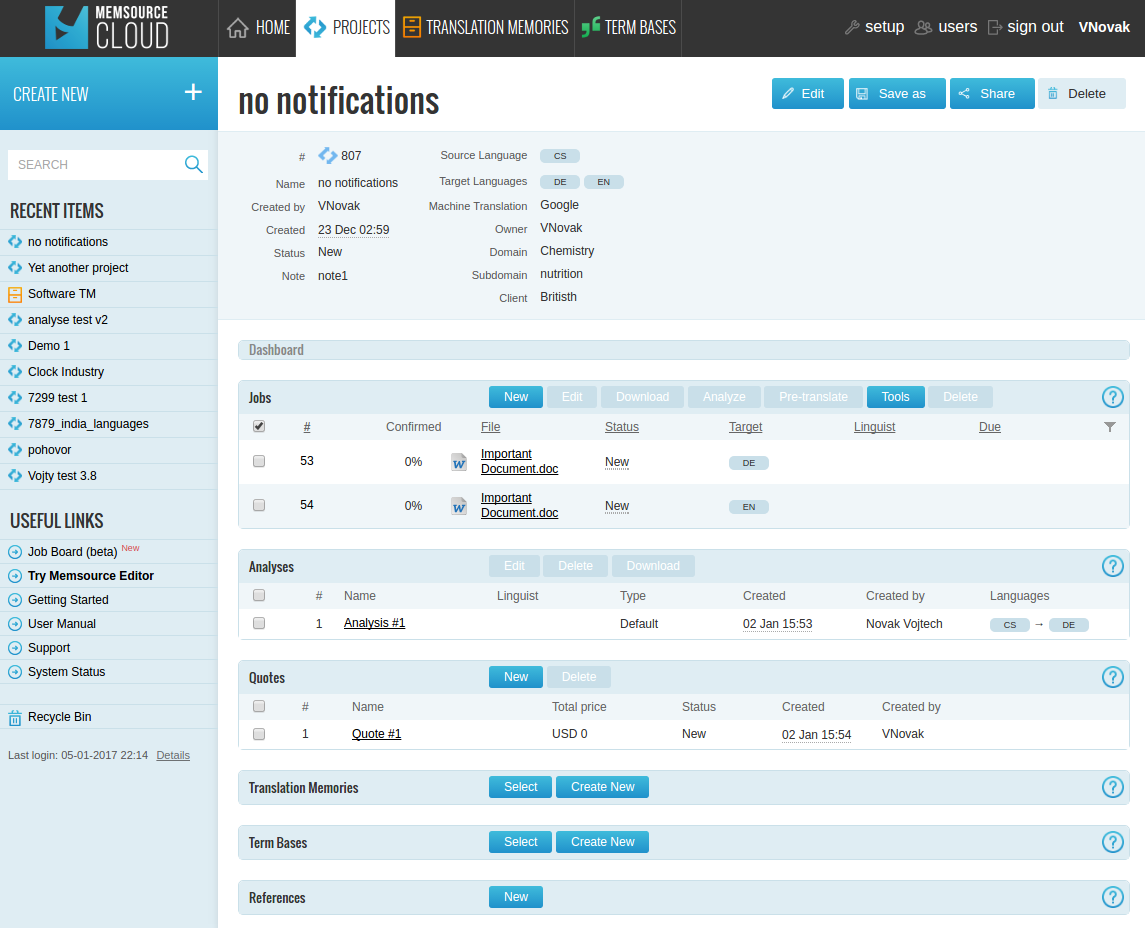
\includegraphics[width=1\textwidth]{pics/cloud/project}
	\caption{A translation project in Memsource Cloud}
	\label{fig:cloud}
\end{figure}

\section{Requirements}
\label{sec:requirements}

The requirements for what the application has to support were determined gradually by a discussion with the Memsource developer team and CEO, followed by discussions with members of the support and product team who understand the customer use scenarios.
The outcome of conducted discussions is described in this section.

First I present a summary of requirements, a more detailed description is also included.

{\bf Summary of requirements}

Non-functional requirements
\begin{enumerate}
	\item app has to run on iOS and Android and be stable
	\item app should be written using technologies already used in Memsource
	\item UI components should have a platform-native look
	\item UI transitions have to feel smooth
	\item UI follows the design guidelines of both platforms
	\item app has to be intuitive to Memsource users
	\item app should keep number of API request minimal, to save resources
	\item the software has to be maintainable and testable
	\item use external software packages only if their license is suited for commercial use
\end{enumerate}

Functional requirements---the app has to:
\begin{enumerate}
	\item use Memsource API to acquire the content
	\item support Memsource project manager and linguist roles
	\item support multiple users logged in at the same time and allow to switch between accounts
	\item list projects and allow to filter them
	\item list jobs and allow to filter them
	\item support adding jobs and projects
	\item allow to edit projects and jobs
	\item store user credentials in a secure manner
	\item support error reporting 
	\item present its UI in English only
\end{enumerate}

In some cases, the tools developed by Memsource are complex so that they support different user needs (for example lots of import options for translation jobs). We do not want to bring all this complexity to the mobile application and thus needed to find only the features we wish the mobile app to include at the start. 


Follows a detailed description of requirements:


\begin{enumerate}
	\item User requirements
	\begin{enumerate}[label*=\arabic*.]
		\item The app will target smartphone devices and a narrow group of users---professional users of Memsource Cloud who understand its features. 
		\item The app has to support the project manager and linguist user roles 
		\begin{enumerate}[label*=\arabic*.]
			\item App has to support multiple users being logged into the app
			\item App will display content for only one user at a time and there will be a simple way to switch between users (i.e. set the active user).
			\item The number of added accounts will be limited to a maximum of four.
		\end{enumerate}
	\end{enumerate}
	
	The situation when a single Memsource user has several accounts is not common, but it is not unheard of (This does happen to users who work for several translation agencies.). This will make working with several user accounts easier, without the need to log in and out or use several browser windows as is the case when using a computer. Currently, the API uses a token for authentication and this token is sent together with all requests. It is thus possible to make such requests for multiple users from the same device. Note that the API is available to only some of the Memsource editions.  
	
	\item Content requirements
	\begin{enumerate}[label*=\arabic*.]
		\item The app will load all its content through an API which is provided by Memsource. In cases where a new API is needed, it will be developed.
		\item The app has to keep the number of API requests as low as possible so that the phone's and the servers' resources are not overused.
		\item The first screen should render within 4 seconds after starting the app.
	\end{enumerate}
	
	It follows that we assume the user will have internet connection available on their device at all times when the app is used to create new content and fetch the up-to-date data. 
	
	Compared to the web-based service, the app will only support selected features, to keep its UI simple and easy to work with. At the same time, it should follow the patterns users know from the web version to avoid confusion. More specifically: 
	
	\item Functionality requirements
	\begin{enumerate}[label*=\arabic*.]
		\item Functionality for PM users 
		
		\begin{enumerate}[label*=\arabic*.]
			\item The app has to support logging in for Memsource users whose role is project manager (PM).
			
			\item Project-related requirements
			\begin{enumerate}[label*=\arabic*.]
				\item App has to support listing projects based on their status (my projects, all, overdue, in progress). The list of projects should contain relevant information (name, customer, due date) for each project.
				\item App has to offer project search using the project name, when the project was created (last 24 hours, last 3 days, last 7 days, last 30 days), the client, the project owner and due date.
				\item PM has to be able to create a new project where they have to able to enter a predefined template from which project can be created, project name, client, domain and subdomain, business unit, source and target languages, due date and note.
				\item App will support deleting projects.
				\item App will support editing projects. The same project properties which are supported by the app when creating a new project will be supported for editing, with the addition of project owner.
				\item The app will allow the PM see project details (name, user who created the project, date when created, status, due date, source and target languages and project owner).
				\item App will support adding existing Translation memory and existing Term base to a project.
			\end{enumerate}
			
			\item Job-related requirements
			\begin{enumerate}[label*=\arabic*.]
				\item App will provide means to show a list of jobs contained in the project, showing relevant information for each job---job name, linguist name, due date, target languages and status.
				\item PM has to be able to create (upload) new translation jobs from document providers available on the platform.
				\item Adding jobs to project from an email attachment also has to be supported.
				\item When adding a new job, user will be able to enter the target languages, select due date, enter linguists for the job and have the option to notify them of the new job.
				\item After a job is uploaded, user has to be informed about it. Similarly, user has to be informed about unsuccessful file uploads.
				\item App should only support creating jobs from the most common file types (MS Word, Excel, Powerpoint and HTML).
				\item User needs to have the ability to select individual job, as well as several jobs, to download, edit and delete them. Editing consists of changing the linguist, status and due date.
				\item Similarly to searching and filtering of projects, the app will allow to filter jobs by name, status, target language, linguist and due date.
			\end{enumerate}
			%\item The application will not cover support for translating, i.e. Memsource Editor will not be a part of it since we found that it is overly complex to be used on a small screen of a mobile device.
			
		\end{enumerate}
		Note: The advanced project creation options for machine translation, analysis and other which are visible in Memsource Cloud, will not be included.
		
		\item Functionality for Linguist users
		\begin{enumerate}[label*=\arabic*.]
			\item The app will support listing projects that are visible to the linguist, filtered based on status (new, accepted, completed). The list will contain relevant information---name, date created, owner, and source and target languages.
			\item Linguist will be able to open a project, download or preview selected jobs and change their status (accepting or rejecting and marking them as completed). 
			\item Same as with a PM, linguist will have the ability to search based on job filename, status, target languages and due date.
		\end{enumerate}
		
	\end{enumerate}
	
	
	
	\item Other requirements
	\begin{enumerate}[label*=\arabic*.]
		\item It is important the app be developed for at least the two major mobile phone platforms, that is Android and iOS.
		\item The app must be developed using programming languages that Memsource developers are already familiar with, that is one or more of: Java, Groovy, C++, JavaScript or any other technology if it brings substantial benefits.
		\item For the user, the app should look and feel as close to a native app as possible.
		\item The application has to support error reporting to allow Memsource continually improve the user experience, app stability and addition of new features.
	\end{enumerate}
	
\end{enumerate}
~


\section{Analysis of Platforms and Development Tools}

Today's market of mobile devices is largely divided between two platforms---iOS and Android. With 80.7\% for Android and 17.7\% for iOS, these two alone made up more than 98\% of worldwide sales in 4Q15, according to Gartner \cite{gartner}. Windows Phone comes third with 1.1\% of sales. Interestingly, in its March 2016 report, Kantar Worldpanel shows the sales vary greatly among different states \cite{kantar}. For example, while iOS has a sales share of 56\% in Japan, it only has 17.8\% in Germany. In 1Q2016, Android was growing in Europe, at the expense of iOS and Windows Phone, whose sales had been dropping in the UK and France where Windows Phone was historically relatively successful. The data from 3Q2016 shows growing Android sales: 86.8\%, 12.5\% and 0.3\% for Android, iOS and Windows Phone, respectively, according to IDC \cite{idc:marketShare} and a report from Gartner \cite{gartner2} shows very similar numbers.


Since we are looking for a solution for creating apps for more than just one platform, I continue with describing the state of the art of multiplatform development tools.

\section{Xamarin}

Xamarin is a framework for developing native apps for iOS, Android and Windows Phone. The company was founded in 2011 and was acquired by Microsoft in 2016. All of Xamarin is now open-sourced on GitHub \footnote{https://github.com/xamarin}. 
Xamarin divides into four main parts: Xamarin.iOS, Xamarin.Android, Xamarin.Windows and Xamarin.Forms. The first three offer access to native APIs for the particular platforms, where Xamarin stresses that ``Anything you can do in Objective-C, Swift, or Java you can do in C\# with Xamarin'' \cite{xamarin:homepage} When using these, the developed solution consists of one project per supported platform (which contains the platform-specific code --- mainly the UI) plus single project whose code is shared and contains the business logic. Reportedly, this approach can result into about 75\% code reuse \cite{xamarin:codereuse}. Xamarin.Forms is an attempt to bring code reuse event higher, usually more than 90\% \cite{xamarin:codereuse} by sharing also the UI code.

As explained, UI in Xamarin can be either defined specifically for each platform within the platform's application project or cross-platform using Xamarin.Forms \cite{xamarin:forms}.

Taking the first way is recommended for apps with interactions that require native behavior, apps which use many platform-specific APIs or cases when custom-tailored UI has higher priority than code sharing. With this approach, each app has its own UI defined in C\# code or XAML (an XML-like sytax for UI description) which can be done in a graphical UI designer.

Using Xamarin.Forms is best for apps that require little platform-specific functionality and apps where code sharing is more important than custom UI. Xamarin.Forms UI can be done either in C\# or in XAML but without the support of UI designer.

Development with Xamarin is done under Windows or OSX and the language of the framework is C\#. The code must be built and sent onto a device or emulator, which can take a considerable amount of time. Development and debugging is best done in Visual Studio on Windows. Xamarin allows to write the code shared by all platforms in the form of a Shared Project or a Portable Class Library \cite{xamarin:sharing_code} which are described in the following sections. 


\subsection{Shared Project}

Shared Project is the simplest way to share source code between platforms. This way, a cross-platform app that supports Android, iOS and Windows Phone would require an application project for each platform and additionally, there would be a Shared Project for the code common to all projects.

The code within a Shared Project can be branched into platform-specific parts using compiler directives (e.g. using \#if \_\_ANDROID\_\_). The application projects can also include platform-specific references that the shared code can utilize.
The downside to this approach is that a Shared Project has no output assembly. During compilation, the files are treated as part of the referencing project and compiled into that project's DLL. This does not allow to distribute the code from Shared Project as an independent library.

\subsection{Portable Class Library}

Portable Class Library addresses the fact that Shared Project cannot be distributed as a standalone library. Portable Class Library offers the possibility to distribute it independently of the mobile app.

The disadvantages are that it is not possible to use compiler directives to reference platform-specific features and the fact that different platforms often use a different subset of the .NET Base Class Library (BCL) and therefore only such subset is available to use. This, to some extent, can be circumvented by the Provider pattern or Dependency Injection. That way, the actual implementation is coded in the platform projects against an interface defined within the Portable Class Library.


\section{React Native}

React Native (RN) \footnote{https://facebook.github.io/react-native} is a counterpart of the popular web development library React and is also developed by Facebook which uses in several production apps and ``will continue to invest in it'' \cite{rn:invest}. It was first released in 2015, which makes it the youngest among the covered solutions. React is popularized under the slogan ``Learn once, write anywhere.'' \cite{rn:invest}, as opposed to e.g. Java whose goal is that one codebase runs anywhere, this means that once a developer learns React, she can use her skills to write apps for multiple platforms (web, Android, iOS, etc.) using just React, but not necessarily with a single codebase.

React originally started as a tool for describing user interfaces for the web, and rapidly became popular within the web development community. However, it was recognized that React's usage was not limited only to web.

React describes the user interface through reusable components which tell what the UI is supposed to look like. It is then the matter of transforming the description into a user-facing UI. On the web, this is the task of React-DOM \cite{learningRN} which uses the Virtual DOM tree as a layer of abstraction between the developer's code and what is rendered in the browser. When programming mobile apps, this abstraction is handled by React Native \cite{learningRN}. At this point, it is important to state that the UI rendered with React Native is not running in a WebView but is built from the native UI elements of the platform in question (i.e. \texttt{View} on Android and \texttt{UIView} on iOS), which makes it different from the longer-established hybrid development environments which also use JavaScript as their programming language. 

RN application code is written in JavaScript which runs in JavaScriptCore engine on the device \cite{rn:jsenviroment}. RN features what is called the \textit{bridge} \cite{rn:bridge}. The bridge is in turn responsible for bridging the calls onto the native platform APIs and back. This way, user can access any native functionality and get information back in a callback or promise payload.

When developing with RN, the developer creates or makes use of ready-made UI components and uses them to compose the application UI. The components are written in a combination of JavaScript and XML tags, called JSX. Optionally, Flow \footnote{http://flowtype.org/}, a static type checker for JavaScript can be used. Also supported although not so frequently used are languages that transpile to JavaScript, such as TypeScript \footnote{https://www.typescriptlang.org/}. From developer's point of view, important features of RN are its live and hot reloading \cite{rn:hotreload}. Live reloading \index{live reloading} enables the developer to apply code changes to the app running on a device or in an emulator quickly. Live reload in fact takes about five seconds on my development machine. This is a tremendous improvement over traditional native development, which until recently---with the introduction of Instant Run to Android Studio---suffered from the slow process of building an app and loading it into a device or emulator.

The other feature called Hot Reloading \index{hot reloading} offers essentially the same functionality as Live Reloading with the advantage of being faster and preserving the application state---the screen displayed before and after the Hot Reload is the same---thanks to which the developer does not need to navigate through the app to the screen where the change is being done. This is especially helpful for making changes to the UI layout and styles because Hot Reload needs only about one second to take effect. These features can significantly accelerate app development and improve the developer experience. The downside of Hot Reloading is that it mostly works for simple changes in the UI but fails when modifications are more in-depth.

Debugging RN is accomplished through running the code in Chrome browser or external debugging tools (such as those included with Visual Studio Code or Webstorm) where user can set breakpoints and work with code similarly to working in web development. In this case, all the JavaScript code runs within Chrome's V8 engine itself and communicates with the phone or emulator via WebSockets \cite{rn:debugging}.


\subsection{Native Modules}

When a developer needs native functionality which is not already provided by RN, they may find such functionality already implemented by the community which surrounds RN. In such case, the component is available through the Node package manager (npm).

In case the functionality is not yet implemented, the developer can create a native module \index{native module} \cite{rn:nativemodules} for it. Native module consists of code written in Java (for Android) and Objective-C (or Swift) for iOS which implements the desired functionality and of JavaScript code that will expose the native functionality to the app's JavaScript code. The native code is invoked from JavaScript through the RN bridge and results (if any) can be passed back by a Promise or callback. Native modules give developer the freedom to implement any functionality desired, as long as it is available on the underlying platform, but have the downside of needing to code both for iOS and Android in the language of the platform.


% pridani do indexu: \emph{affine}\index{affine}
\section{Ionic}

In version 2.RC4 as of 1/2017, Ionic \footnote{http://ionicframework.com} is another successful framework for developing cross-platform mobile apps which was initially released in 2013. Ionic is a hybrid framework, meaning an app created with it runs in a WebView, same as a website would---with the important difference that it can also use the native device APIs. Ionic supports iOS, Android and Windows Phone.

Just like the aforementioned frameworks, Ionic is open source and offers a set of mobile-optimized components written in HTML, CSS and JavaScript. Ionic 2 integrates with Angular 2, a framework for web development from Google. Ionic has put a lot of work into providing components that are styled (more or less) according to each supported platform, thus saving the developer's time by not having to spend valuable time by styling everything in the UI. Compared to React Native and Xamarin, Ionic gives less flexibility in customizing the app per platform. With Xamarin and RN, developer can make the app look and behave quite different (at the expense of writing more code) while this is limited on Ionic. Depending on the particular app context, this can be both a downside or a benefit.

Ionic 2 developer can optionally choose to develop in TypeScript, which is a language that compiles to plain JavaScript. As its name reveals, the most important feature of TypeScript is the addition of types to JavaScript. This can reveal errors before they happen, and gives extra information to both the developer and IDE (Integrated Development Environment) which therefore can offer better code completion. TypeScript is basically a competitor of Flow.

Ionic runs inside Apache Cordova \cite{ionic:cordova}, a mobile application development framework which provides access to native platform features \cite{cordova:intro} such as camera, sensors, filesystem or contacts. Access to arbitrary features can be allowed through plugins, which are composed of a single JavaScript interface used on all platforms, and platform-specific code code which is called from JavaScript. In this respect, Cordova Plugins are similar to native modules in RN.

Ionic involves more than just mobile app development. It offers features like ionic lab, which allows to run iOS, Android and Windows Phone version of an app one next to the other in the browser. There is also the Ionic Market, which contains lots of starter templates and themes. Ionic's View app allows developer to easily share apps with customers and testers. Ionic Creator is a prototyping tool where developer can drag and drop components to create a simple app and even export it as an Ionic app.

Also, with live reloading, the iteration process is a lot faster than traditional procedures that involve compilation.


\section{Conclusions}

There is currently a very strong competition in the area of multiplatform mobile app frameworks and choosing one is no easy task. All of the researched solutions are very capable. 

After developing simple proof-of-concept apps using the three described frameworks I first ruled out Xamarin. Although C\# can be considered a very mature and powerful language, the reasons for ruling Xamarin out were the need to write UI twice - which would involve learning the specifics of Android as well as iOS. We did not want to use Xamarin.Forms because we were uncertain about whether it would not limit us and the available demonstrations apps written using Xamarin.Forms did not make a very good impression on me (the official Xamarin Evolve conference app took long to start and repeatedly froze on my Nexus 5 phone). Moreover, Xamarin's slow development iteration cycle, for me, felt like a big drawback.

Ionic 2 is a popular framework. After creating simple application in it, I could not help but notice very slow startup times: between 7 and 10 seconds for a very simple app. This issue was confirmed by posts in the community forum \footnote{https://forum.ionicframework.com/t/ionic-2-speed-up-boot-time/46372/111} and according to an Ionic representative, the startup time will be improved in future releases. After installing several apps developed in Ionic we noticed not all of them work on all devices (probably due to cpu family), which left me with mixed feelings. The advantage of Ionic 2 surely lays in its maturity, strong community and lots of readymade UI widgets styled differently for each platform.

% However, as of January 2017, the Ionic Conference app

React Native was chosen after difficult comparisons. Its advantages are that it is backed and used by Facebook, it is being developed at a quick pace and has a growing community with lots of components available or in development. It also provides greater UI flexibility than Ionic, better performance, and the ability to easily communicate with native code is a need for our use case since the app will have to deal a lot with files (background file uploads, downloads, importing them into the app). Most importantly, RN does a very good job at transforming the React code to the native views. Obvious disadvantage is its immaturity and probably the need to work harder to get eye-appealing designs because unlike Ionic, RN does not offer styled UI components ready to be used but only the essential components with no multiplatform interface. 

Table \ref{tab:comparison} provides a quick comparison of the described libraries or frameworks against selected criteria. Plus sign (+) denotes positive rating, while zero (0) and minus (-) denote neutral and negative rating.

\begin{table}[htbp]
	\centering
	\caption{Comparison of the considered multiplatform development tools}
	\label{tab:comparison}
	\renewcommand{\arraystretch}{1.2}
	\begin{ctucolortab}
	\begin{tabularx}{\textwidth}{XYYYY}

		\textbf{Platform} & \textbf{Xamarin} & \textbf{Xamarin Forms} & \textbf{Ionic 2} & \textbf{React Native}\\ \hline
development speed          & -                           & -                                 & +                           & +                                \\ \hline
performance                & +                           & +                                 & -                           & 0                                \\ \hline
maturity              & +                           & 0                                 & +                           & -           \\ \hline
platform-specific behavior & +                           & -                                 & -                           & +                                
      
	\end{tabularx}%
\end{ctucolortab}
\end{table}%





\chapter{Design}

After analyzing the task and collecting the requirements, this chapter will go through the design of initial paper prototypes as well as higher fidelity software prototypes. I will also describe the architecture of the mobile application which is crucial for successful development, future extensions and maintenance. I will talk about different components that the application is composed of and how they cooperate to achieve desired functionality. This chapter contains several UML diagrams, all of which are simplified.

\section{Application Structure}

The application requirements give a thorough description of the features the app will offer. Upon the requirements I have designed the application navigation structure that I'd like to follow. Figure \ref{fig:structure} shows the hierarchy of the app's screens with somewhat simplified screen transitions. The root of the navigation is the Project List screen which will show lists of projects. For each project, the hierarchy then goes deeper to allow user to view further project information and to work with jobs, translation memories and term bases. Another application entry point is the screen for adding a job from an external application (e.g. from Mail or from a filesystem browser application).

\begin{figure}[]
	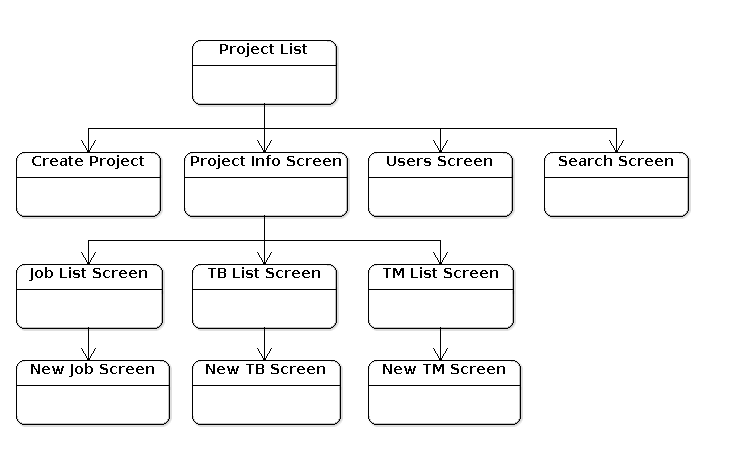
\includegraphics[width=1\textwidth]{argoUml/structure}
	\caption{Structure of the app's screens.}
	\label{fig:structure}
\end{figure}

\section{Prototyping}

Based on the collected requirements, a set of mockups was constructed. Some of these were later used to construct a prototype for an Android device that was used for tests with users. Both the mockups and the prototype consider the project manager role because its feature set is a superset of the one of the linguist role.

The mockups were discussed with employees of Memsource support team. Different ideas of presenting information to the user were brought up and consulted. Memsource support members provided feedback and deeper insight on how different features are used and whether they are needed. Understanding the workflow was important to designing the final mockups.

In the end, the prototype largely follows the structure of Memsource cloud, but it is simpler in terms of the number of supported options and gives off Android platform feel. The following pages contain several figures that present selected mockup screens.



\begin{figure}[]
	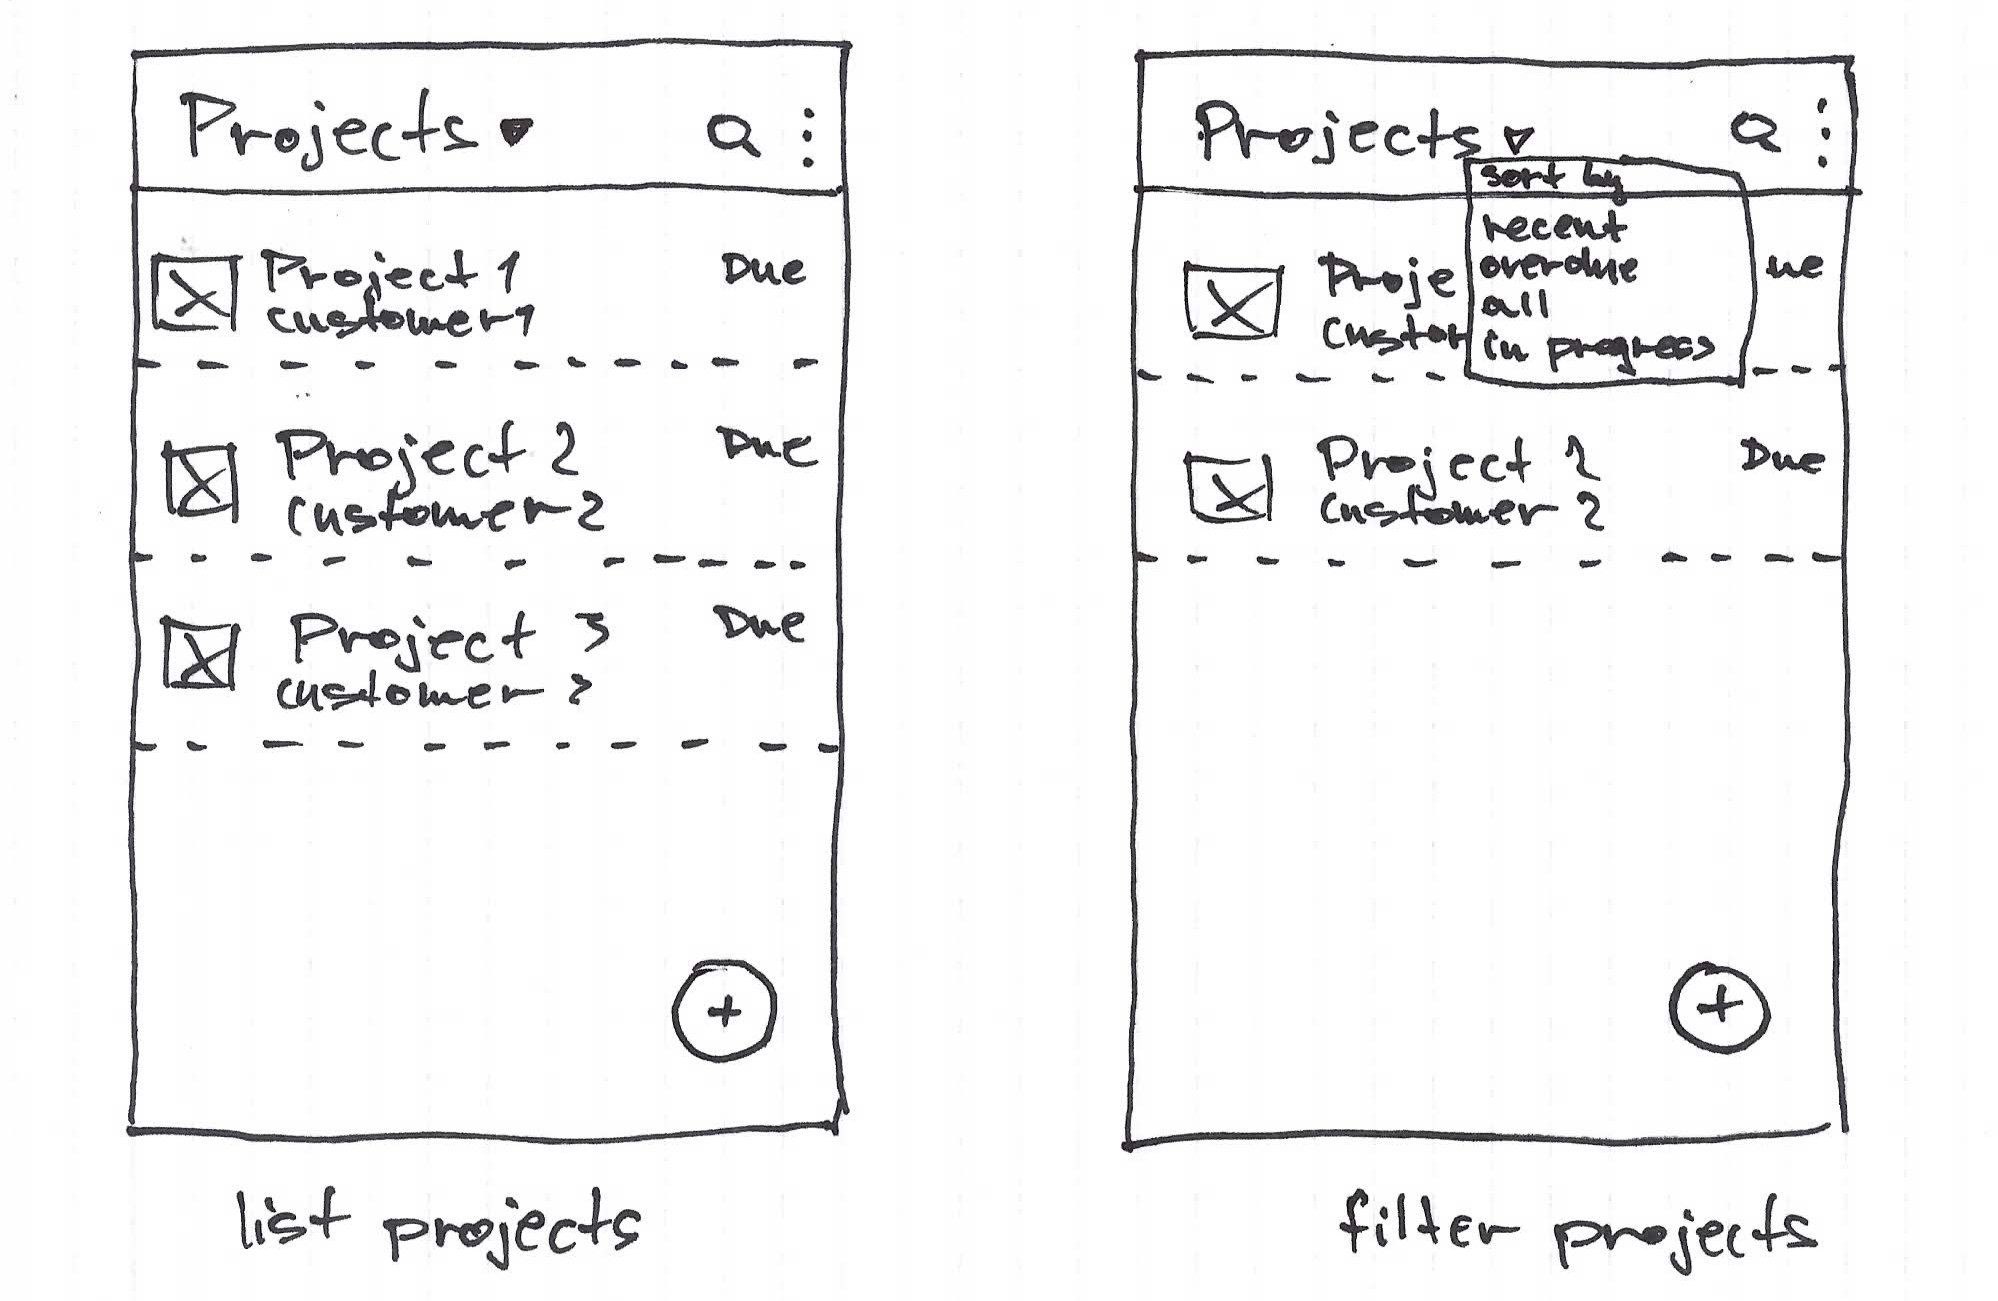
\includegraphics[width=0.7\textwidth]{pics/projects1}
	\caption{Mockups showing the project list screens. Second screen shows the chevron active, where user can filter displayed projects.}
	\label{mock2}
\end{figure}

\begin{figure}[H]
	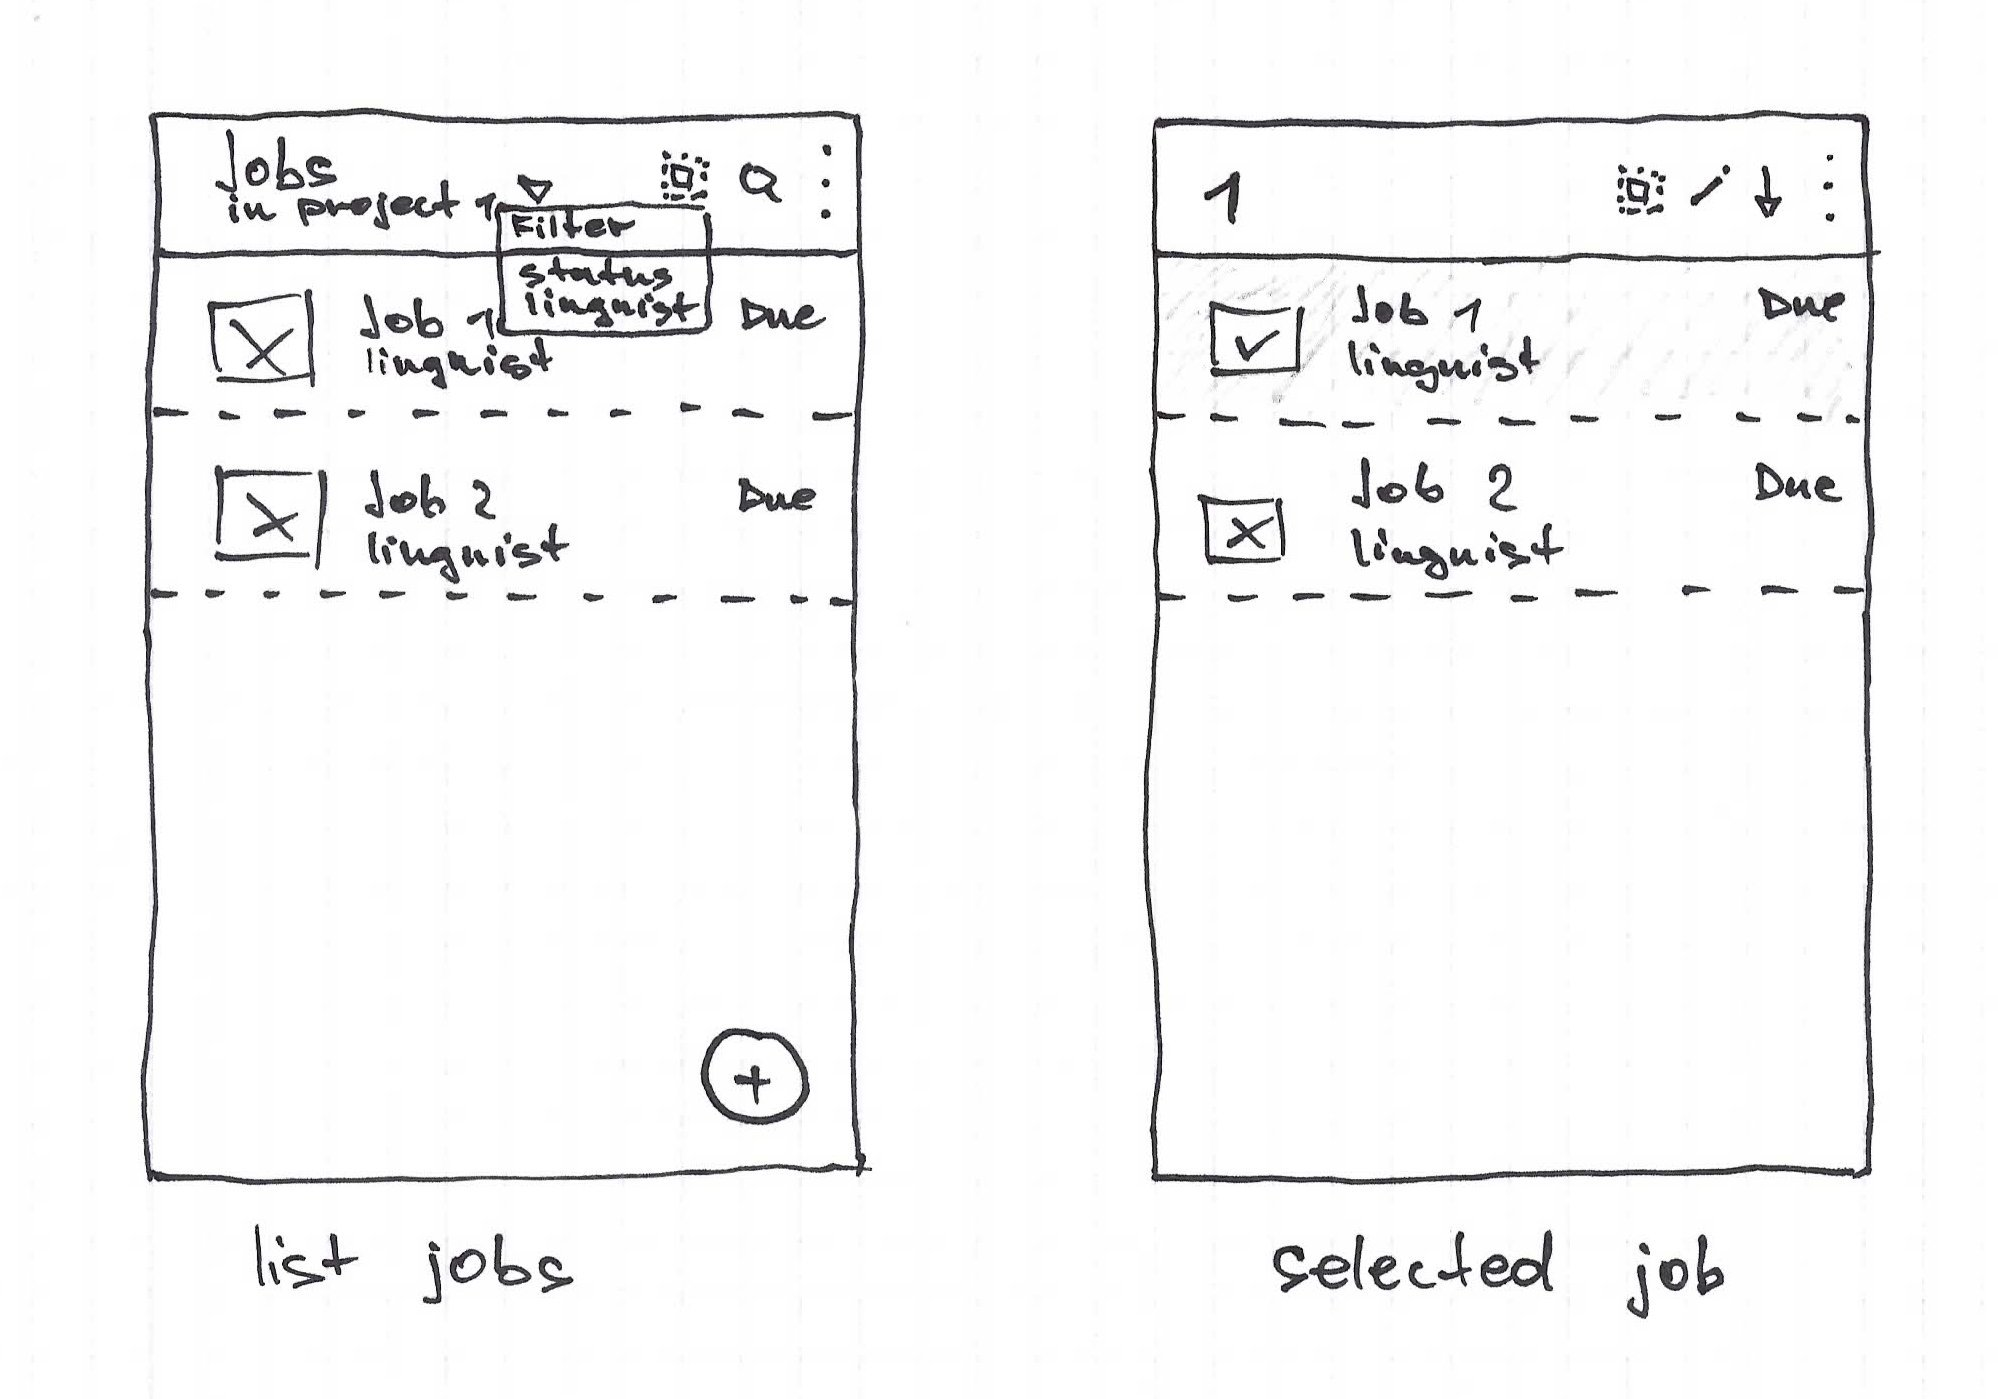
\includegraphics[width=0.7\textwidth]{pics/jobs1}
	\caption{Job list (left) and a mockup where ``Job 1'' is selected and different actions are available for it (right).}
	\label{mock3}
\end{figure}

\begin{figure}[H]
	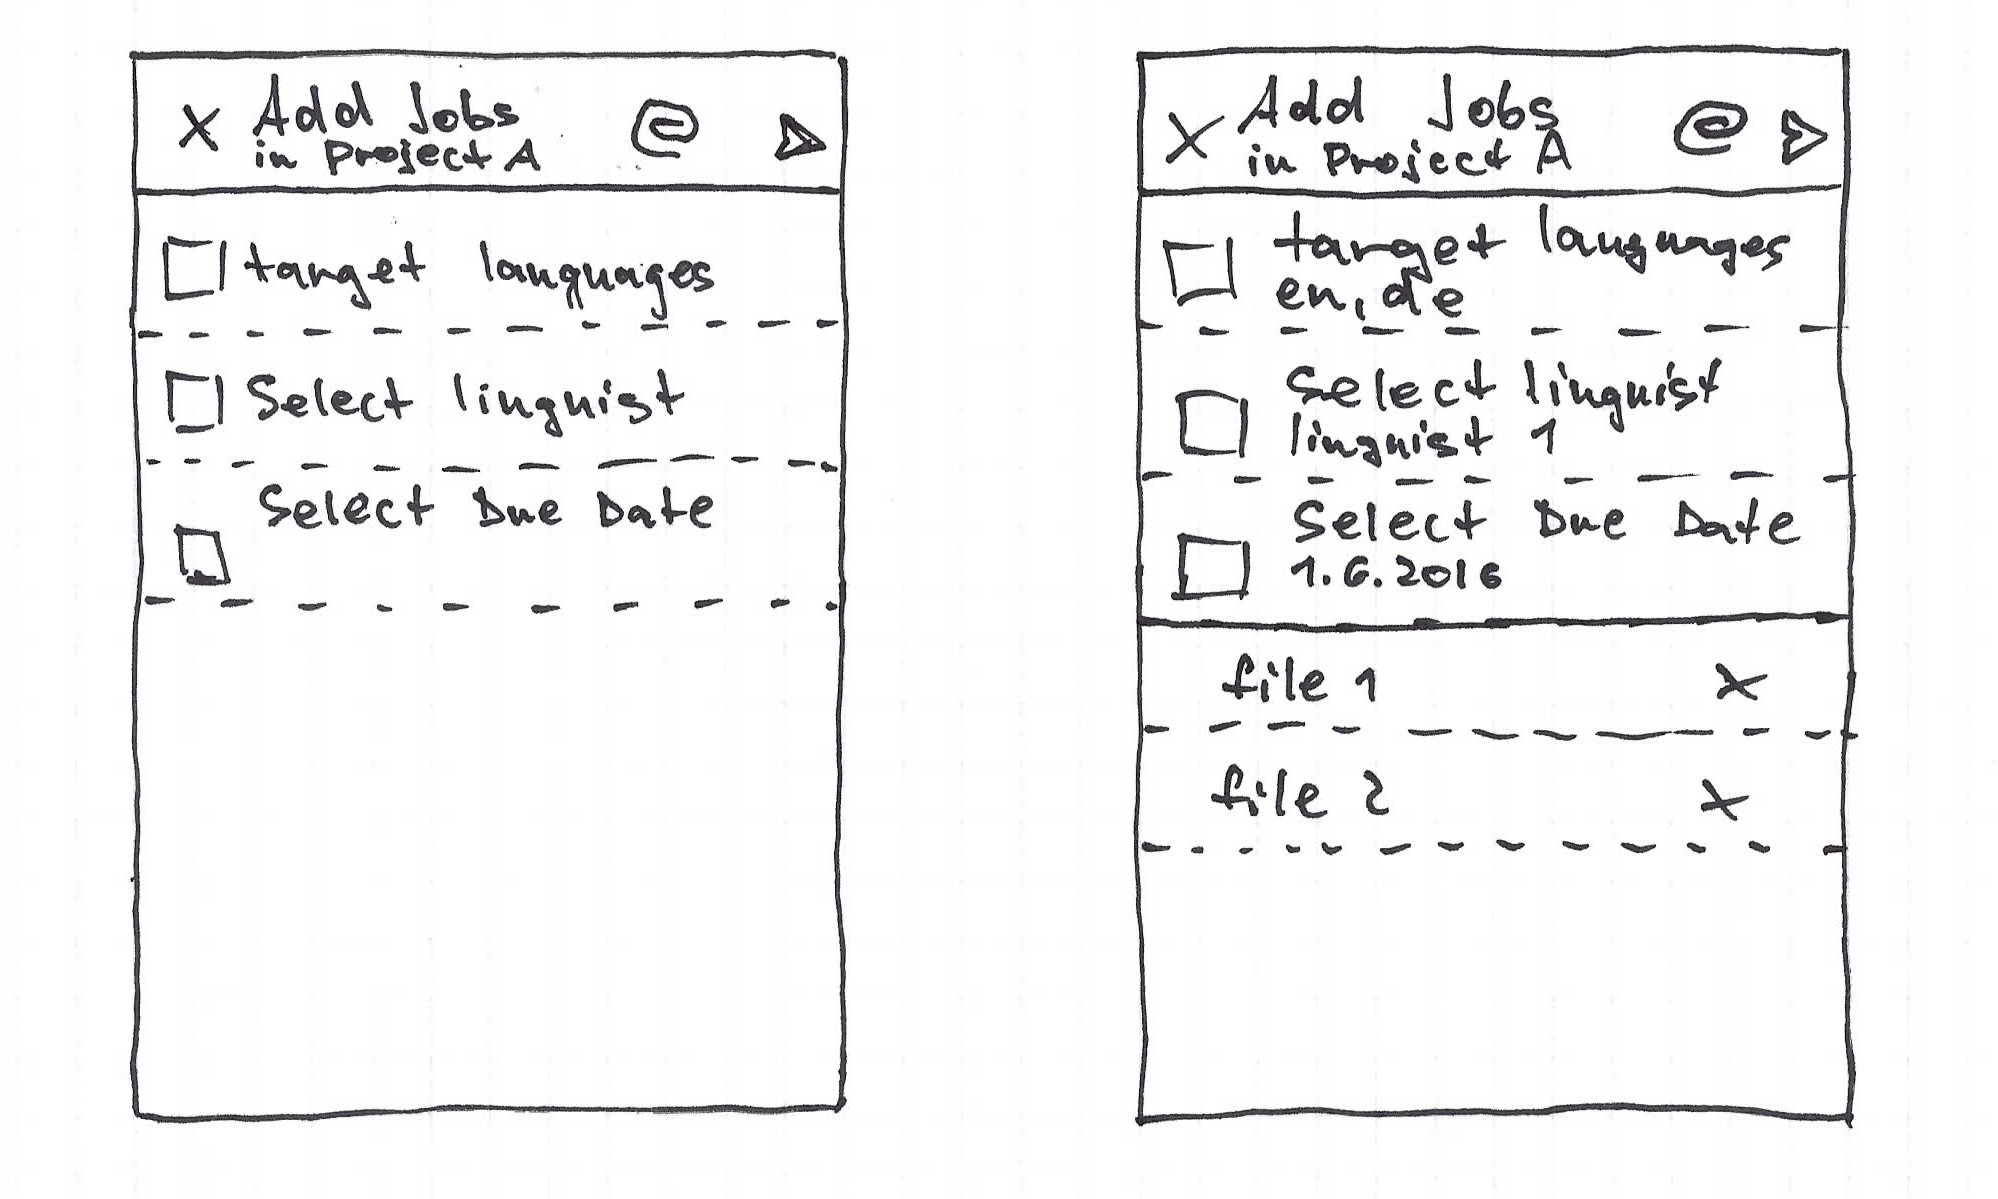
\includegraphics[width=0.7\textwidth]{pics/addJobs}
	\caption{Adding a new job to a project.}
	\label{mock4}
\end{figure}


Figure \ref{mock2} shows design of the project listing. There are controls for creating a project, searching, filtering (using the chevron) and getting the important information about user's projects. In figure \ref{fig:proto} you can see how filtering the projects changed in the final prototype. 

Figure \ref{mock3} shows a mockup of an opened project with translation jobs listed (first screen). The second screen shows a job being selected and the consequent changes in the navbar: the user can choose to edit, select all or download job. 

Figure \ref{mock4} contains the screens for adding a new job to a project from within the application. The figure shows two states of the same screen, first screen is waiting for user to enter needed information, the second displays the state when the information is entered, along with two files chosen for upload. In the prototype, the layout of these screens was preserved, except for division into two tabs: one for uploaded files and second for import settings.



For iOS, which has different interaction patters compared to Android, I created separate mockups of what the UI could look like. The figure (\ref{mock5}) shows the mockup of job listing and handling.

\begin{figure}[]
	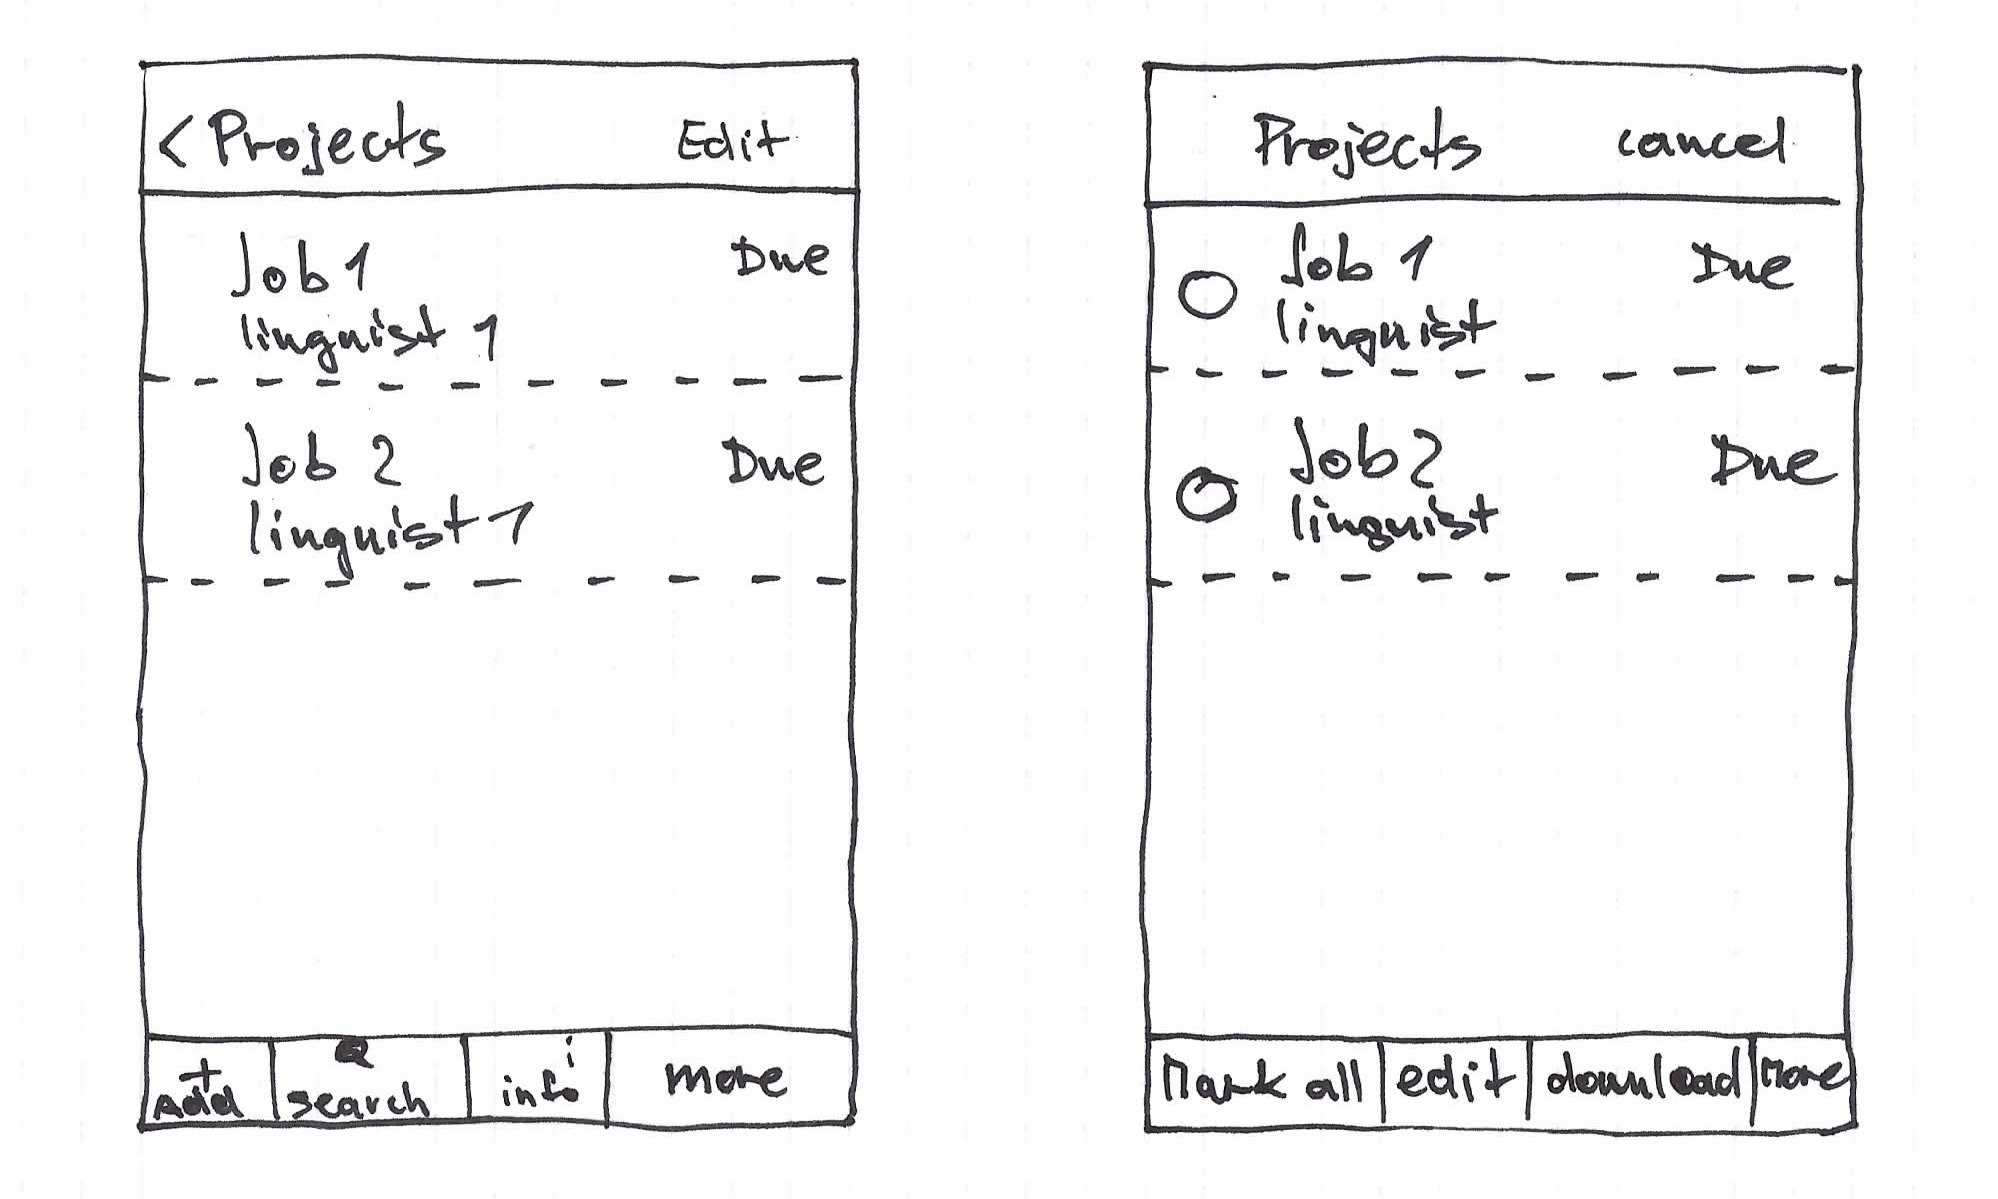
\includegraphics[width=0.8\textwidth]{pics/iosProjs2}
	\caption{Different way of listing jobs within a project on iOS. The second screen displays the state of the first after clicking on the 'edit' button.}
	\label{mock5}
\end{figure}



\subsection{Testing with users}

From the mockups I created a software prototype for Android. The prototype was created using Axure RP 8.0 \footnote{http://www.axure.com/} which is a software for creating different kinds of UI prototypes. There are widget libraries available, which contain ready-to-use Android and iOS UI elements. Figure \ref{fig:proto} show selected prototype screenshots.

To verify the created prototype, I conducted two informal tests with users. Axure provides Axure Share service to share projects, with and Android app \footnote{https://play.google.com/store/apps/details?id=com.axure.axshare} available on the Google Play Store, but this app proved not to be suitable for testing because it does not scale the UI well. Instead, I took advantage of Axure's ability to export created project as HTML which can be viewed directly on the device, for which I used the Kiosk Browser \footnote{https://play.google.com/store/apps/details?id=it.automated.android.browser.kiosk} app which allows to display content full-screen. 

To help keep the users relaxed, I explained the purpose of the application we were about to test and that we were testing only an initial prototype to catch its flaws, and not testing their abilities of working with Android.

The users were given a list of tasks corresponding to a possible walkthrough of the app. The text is following: 

You are a Memsource Cloud user and your role is project manager. Log in using the username ``user'' and password ``pass''. View translation jobs in Project 1 and download job whose name is ``Job name'' onto your device. Then create a new job from the ``document.docx'' which is available on Google drive. For the job, select English and German as target languages, due date as 2nd January 2016, 11:00 am and enter linguist name. You need the file be imported with comments and hidden text. Then, create a new project as new project name, enter ``test project'', select ``client 3'' as the client and select arbitrary parameters for the other options.

The informal testing was conducted in the company offices with two members of Memsource support team who both were owner of a mobile phone running Android. Test was conducted using LG Nexus 5 with the prototype running in the aforementioned Kiosk Browser. The downside of this setup was that the back button of the prototype was not available and in one instance (before adding a new project), this required intervention into the test process and consequent finding that a back button should be added to the navigation bar. Also, the generated html prototype seemed to have issues with entering text into textfields---they were accessible only after a long press instead of a simple tap. I have not found the root cause of this and needed to inform users of this issue before starting the test.

\begin{figure}[]
	\centering
	\begin{minipage}{.5\textwidth}
		\centering
		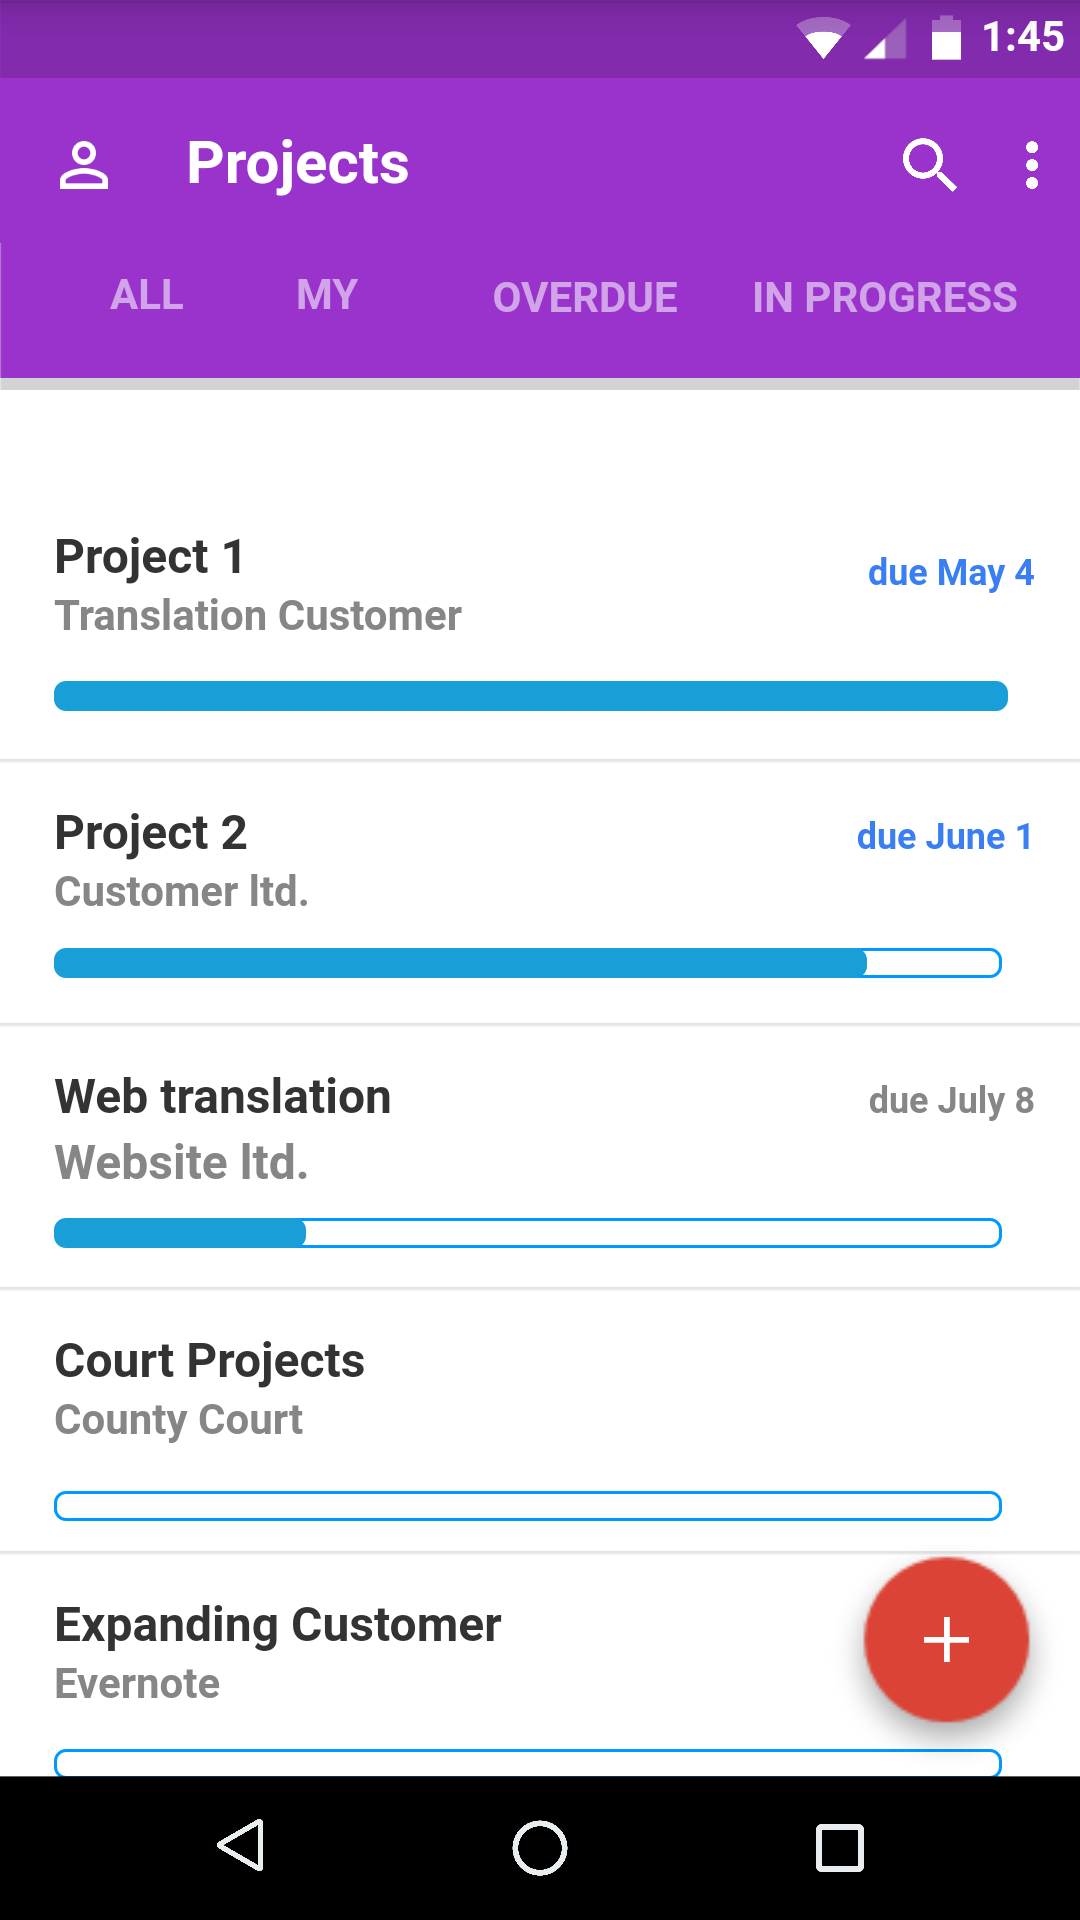
\includegraphics[width=.74\linewidth]{pics/protoProjects}

	\end{minipage}%
	\begin{minipage}{.5\textwidth}
		\centering
		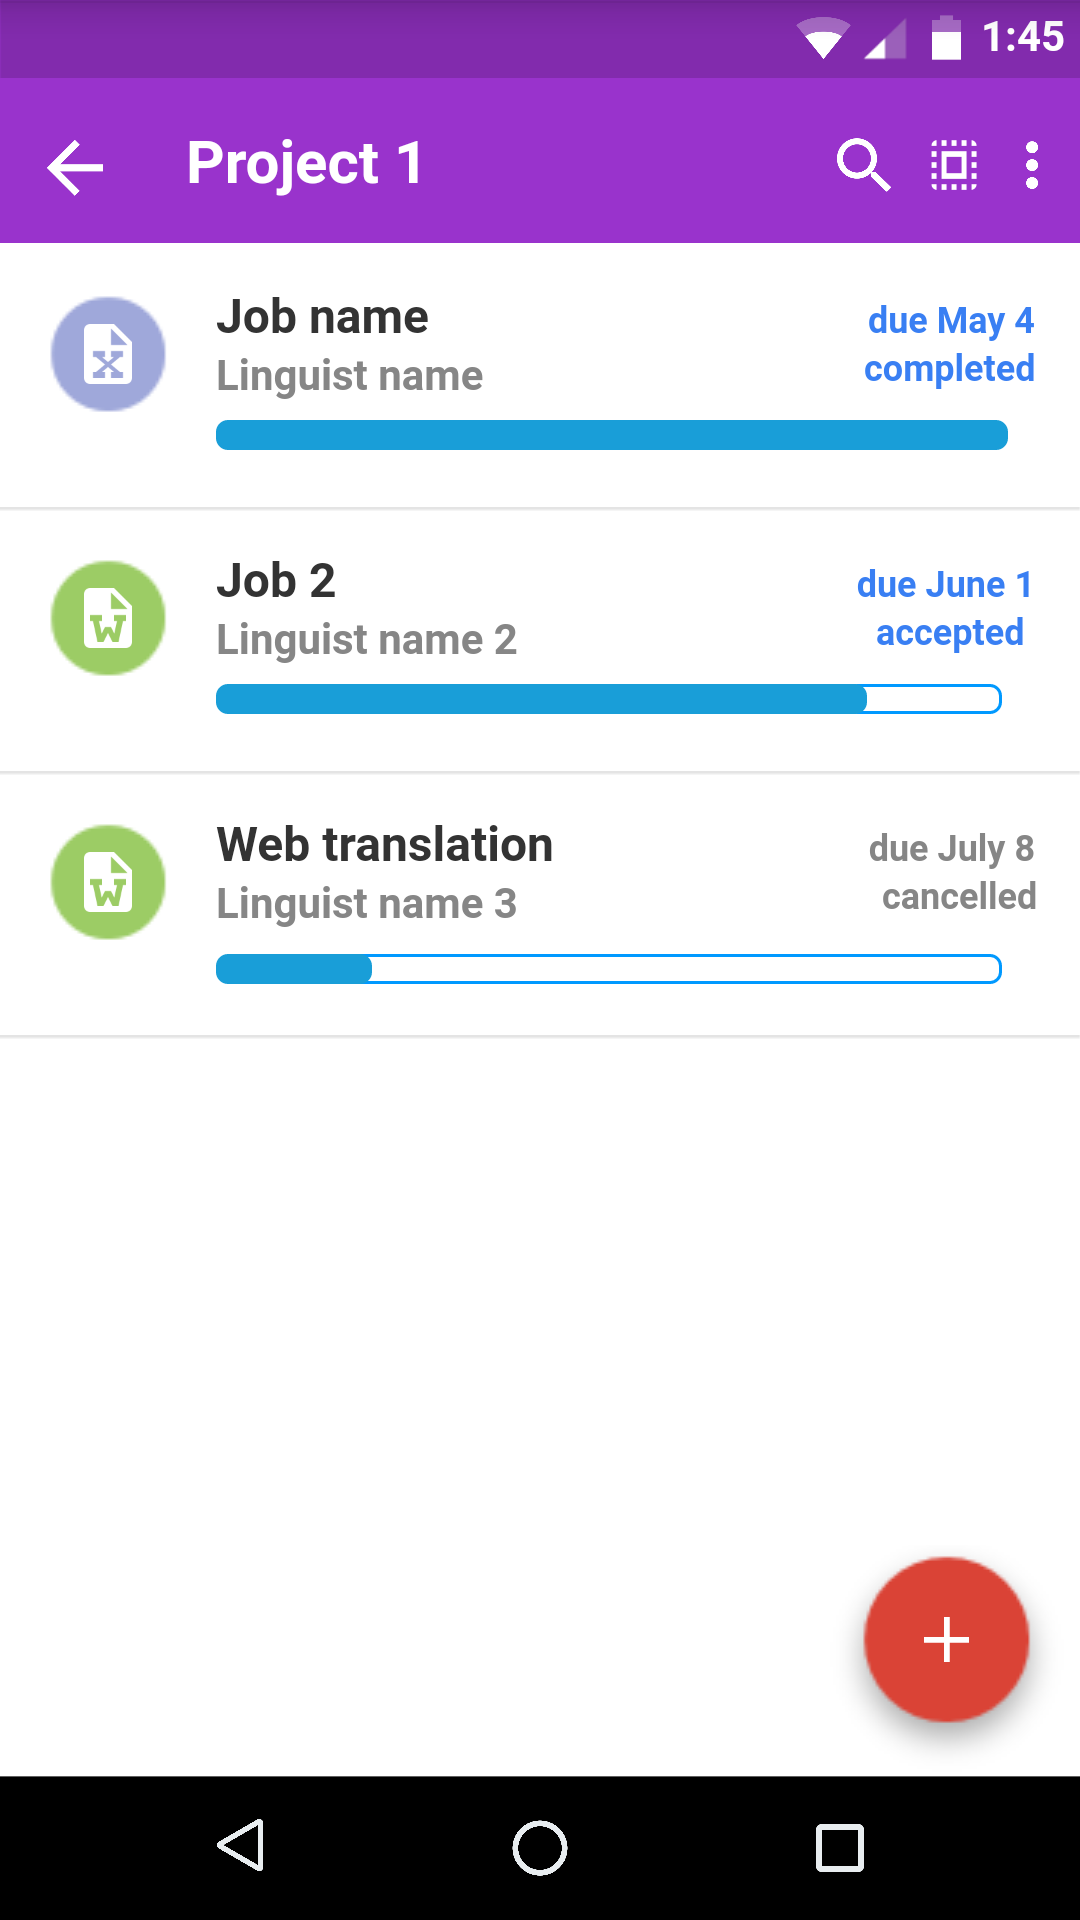
\includegraphics[width=.74\linewidth]{pics/protoProject1}
		
	\end{minipage}
	\caption{Listing projects (left) and jobs in a project (right).}
		\label{fig:proto}
\end{figure}


\subsection{Test results}

The test was completed by both users. However, during the test, two mistakes present in the UI were reported (problem with import options and adding new project). Both users complained about unintuitive icons, which was especially true of the white cloud icons in the upper right corner of the screen. After filling in all information for a new project, one user asked if that was the icon they were supposed to tap.

For the second iteration of testing, I used an improved prototype which fixed the flaws we found in the first iteration. Also, I stopped using the kiosk app and opted for the Axure Share Android app after fixing the scaling issue. The second test was successful and users reported they were satisfied. One tended to play with the prototype beyond the extend of what it was made for and complained some buttons were not functional. I do not consider that a problem, since this was mainly a horizontal prototype with only a particular interaction path implemented.



\section{Application Architecture}

In this section I describe the process of designing the inner workings of the application with respect to the fact that React Native was chosen as the library for implementing the application. This first involves finding a solution for app's state management which may fundamentally influence the architecture.


React Native allows to create user interfaces from the fundamental building blocks of the platform it runs on (\texttt{View} on Android and \texttt{UIView} on iOS) and it also provides means for communicating between the Javascript and native layers. What remains to be chosen is a library that will be used for storing the application state - ie. all of the data fetched from the Memsource API and displayed in the app such as project data, app user information and other. There are several libraries that help solve the problem. The most popular at the time of writing is called Redux \cite{stateOfJS}.

\subsection{Redux}

Redux is built around several core principles:
The entire app state is stored in a single object called the store \cite{redux:store}. The state can be modified by actions which are plain JavaScript objects describing the name and payload of the action \cite{redux:store}. Actions are dispatched to reducers. Reducer is a pure function that takes two arguments: previous state and action, and returns the new state.

Pure function \index{pure function} is a function that always returns the same result given the same parameters and produces no side effects. It is important that the reducer calculates the next state and returns it, without modifying the previous one.
As the application grows, the root reducer function is split into more reducer functions responsible for reducing different subparts of the state. Designing the shape of the state object is therefore key part of using Redux in any application.

Redux requires that the state is not modified in the reducer, which works well with the use of persistent immutable data structures \cite{redux:intro} (PIDS). The most popular implementation of PIDS in JavaScript is Immutable.js. Immutable.js offers data structures that present an mutable interface (such as add() method for an array) but instead of mutating the original object, a new object is returned, so using the reference equality operator will return false.

When changing an object in PIDS, the new object is essentially a copy of the previous one but as much content as possible is recycled from the previous object. Other objects that pointed on the old object need to be copied as well, but objects that do not need to be copied stay unchanged. Implementations of PIDs use Trie data structure to represent common data structures such as arrays using a tree. This is shown in the following figure todo. 

Lastly, Redux provides the redux-react package which allows the React components to "connect" themselves to relevant parts of the state tree and receive the data from them through props.


\subsection{MobX}

MobX is another state management library with growing popularity that has React bindings. MobX uses observable data structures that, as opposed to Redux, are mutable. Its key philosophy is that "Anything that can be derived from the application state, should be derived." \cite{mobx:intro}. Compared to Redux, MobX requires writing less code and while its internals are much more complex because of the change tracking, it offers synchronized state and views out of the box and its API surface is small.

With MobX, the first step is to declare the state and make the relevant parts of it observable. This is usually done in ES6 classes.
The next part is observing the changes in observable data. This is done through tracked functions. MobX tracks the observable data used during the execution of tracked functions and invokes them upon change in that data. 

One of the most important tracked function is \texttt{autorun}. If an observable data used in autorun changes, autorun is re-run. This is the function that is responsible for keeping the React views in sync with the observable state. MobX provides the mobx-react package which includes an \texttt{@observer} decorator which can be used for React component to make them react to changes in observable data, and the decorator makes use of \texttt{autorun} internally.
MobX also provides many other reactive utility functions for more fine-grained reactions. An example of how MobX can be used with React is shown in figure \ref{code:mobx} where a simple React component shows the number of seconds since the code was executed.


\lstinputlisting[label=code:mobx,caption=Using MobX with React]{./code/mobx.js}


After developing a small part of the application with Redux and also MobX, I chose to use MobX for storing the app state. The reasons for choosing MobX were its simplicity and proximity to object-oriented software design which I'm more experienced with. 
Using Redux requires writing boilerplate code to describe the actions and writing the reducers. Also, it is not always possible to dispatch actions that are plain objects - communication with Memsource API, for example, would require dispatching functions that would change the state after receiving data from the API. Working with hierarchies of objects also requires normalizing the application state, similar to how it is done in databases, with ids used as keys for retrieving a referenced object from other parts of the state tree. Apart from Redux itself, this then involves understanding several other libraries such as normalizr, redux-thunk (or other), reselect (optional) and Immutable.js (optional but much recommended).


With MobX, the app will consist of the views which are handled by React, domain objects, which are Javascript objects and some of their properties will be marked as observable or computed (ie. derived from other observables). The domain objects will be stored in domain stores. Stores are objects that instantiate new domain objects, delete the existing ones and provide other necessary functions with regard to domain objects. The last piece of the puzzle is handling communication with the Memsource API.

\section{Client-server Communication}

Communication with the Memsource API will be facilitated through an ApiCaller object whose simplified class diagram is shown in figure \ref{ApiCaller}. The documentation of Memsource APIs is publicly available at the \href{http://wiki.memsource.com/wiki/Memsource_API#API_Reference}{''Memsource wiki''}.

\begin{figure}[H]
	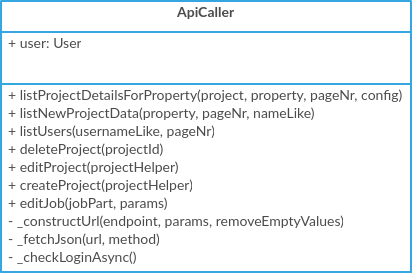
\includegraphics[width=0.6\textwidth]{pics/ApiCaller}
	\caption{ApiCaller class}
	\label{ApiCaller}
\end{figure}


ApiCaller will expose methods that offer CRUD operations over various resources such as project or jobs. All of its methods will return a Promise object which returns the fetched data upon resolving. ApiCaller will be used mostly from the stores and other functions needing API access. The advantage of having an object that will hide the fetching logic inside is easy testability and maintenance - if fetching is done in one place, it is easy to mock and change the implementation if needed. ApiCaller also contains a reference the currently active user, so that it fetches data in the user's name.


\section{Domain Objects and Stores}\label{sec:stores}

There are several core domain objects the application needs to work with. These represent the corresponding entities in Memsource Cloud and will be fetched through the API. These objects are mostly simple data holders, with little logic included in them. 

Domain objects will be stored in stores. Every type of object will have its own store that takes care of saving, editing and deleting the objects and may contain further logic needed to fulfill these tasks.
Figure \ref{Project} shows the Project class and figure \ref{projectStore} shows the store for projects. 

\begin{figure}[H]
	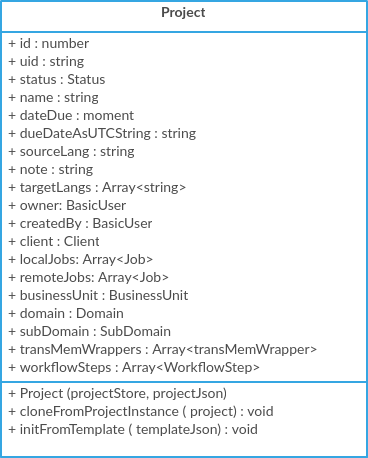
\includegraphics[width=0.6\textwidth]{pics/Project}
	\caption{Project class}
	\label{Project}
\end{figure}


\begin{figure}[H]
	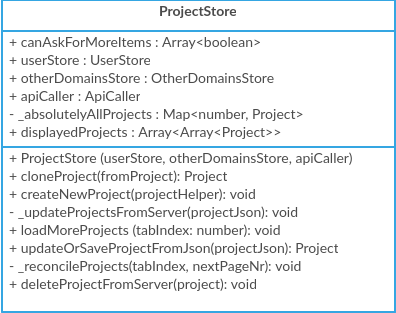
\includegraphics[width=0.6\textwidth]{pics/ProjectStore}
	\caption{ProjectStore class}
	\label{projectStore}
\end{figure}

For tasks such as creating projects or jobs, dedicated objects will be created, with their life span being limited by the sole task they need to fulfill.

\subsection{Representing Users}

Since the application has to support multiple users being logged in (with only one user being active at a time), we need objects for representing individual users as well as the collection of users who are logged in.

For this purpose, the User and UserStore classes are used. User instance contains data such as user name and id, and also user password, token, role and other. It is also the place where the user's search history is kept.

UserStore will contain an array of all users who are currently logged into the app, and a reference to the user which is currently active. Furthermore it will contain methods for creating new user instances and persisting the user information so that it is available upon application startup.


%\subsection{Representing Jobs}



\subsection{Platform-specific Look and Feel}

React Native does not aim to provide developers with a way to run the same code on both platforms, instead it promotes the “learn once, write anywhere” paradigm and allows to create apps for both platforms while writing code using the same syntax.


Due to the nature of how both platforms are interacted with, we need to have an ability to make the user experience different per platform. As an example, take the Datepicker on Android versus the iOS Datepicker, or the Android navigation bar which often offers several actions (some with icons) versus iOS navigation bar which usually contains the title and no more than 2 actions. 
Actions that, on Android, would be included in the navbar, are often presented in a toolbar on the bottom of the screen on iOS, or hidden in an action sheet. Also note how Android works with presses for item selection (for example in the Gmail app or the Downloads app), while this is usually done by an edit button in iOS navbar. The edit button then switches to an edit mode where user can perform their edits. If we want to follow these customs, this requires us to write separate code that would make the UI look and react to user actions differently on each platform, as well as custom code for the item selections and Android back button handling.


React Native offers two ways how to go about platform-specific behavior. First is through the Platform module which gives information about the platform and its version. Another method is to use different file extensions (ie. \texttt{android.js} or \texttt{ios.js}) for components. The appropriate file will then be packed for the JavaScript bundle of each platform. Specifying what component to render by using different file extension is a powerful concept: typically a developer would use this approach for components that will serve the same purpose but need to look differently on each platform. Both files then have the same interface which abstracts away the inner differences. Such approach can be used in a number of components such as buttons, pickers or even a non-component code. I will take advantage of these features to improve user experience and to follow the design guidelines.




\chapter{Implementation}

This chapter describes the implementation of the features that were identified in the analysis. I will focus on the interesting parts of the implementation.

From a higher-level perspective, there are several subparts of the project that need to cooperate for the client app to work well. Firstly, there are the domain objects and stores implemented with the help of MobX. Secondly, there is the view layer created with React Native. The third piece is handling API communication and lastly, there are the native modules for handling job upload (ie. uploading files to Memsource and creating jobs from them) which are the only custom code of the application that is not be written in JavaScript. This chapter explains in depth the solutions to these tasks and issues encountered along the way.


In the following text, I will often use the terms Javascript layer, native layer and asynchronous bridge. When talking about the Javascript layer, I refer to the Javascript code which runs in JavascriptCore engine. By native layer I mean the code that is being executed on the Android’s virtual machine or todo in iPhone. To explain the importance of these terms, let us quickly take a look at an example of how the bridge affects us. 

When React Native communicates between the Javascript and native layers, it uses batched messages that it sends through the asynchronous bridge. This means that if you want (or are forced to, in some cases) to access some value synchronously from one layer or another, it has to be available in that particular layer. In some cases this means a value has to be duplicated on both sides of the bridge and has to be synchronized using a call through the bridge. However, when a value exists on both sides of the bridge, we need some mechanism that will be able to determine which of the two values is the most-up-to-date one. 

As an example, let us consider the textinput component on ios. Because of the design of the platform, the value entered in the textfield has to live in UIKit. We would, however, like to be able to control and read the text input’s value from Javascript synchronously. Imagine a text field into which we start typing “ABC” as input. At time 1, the native UI thread sends the first letter to the JS thread. The JS thread, however, doesn’t pick up the value until the next run of its execution loop. At time 2, user enters B and the UI thread sends the value “AB” is sent to the JS queue. At the same time, the textfield value is set to “A” in response to the update sent from the JS thread. At time 3, user enters C and so the UI thread sends “AC” to the JS queue. At the same time the value “AB” that JS just received is sent through the bridge. In the end, the JS thread receives “AC” and sends it again through the bridge. Both the native and JavaScript layers contain the same value - “AC” but the character “B” has been dropped! The solution implemented in RN involves a counter of input events of the text field which is sent through the bridge and the value of the textfield is not changed unless the counter number received from JS is higher than the one stored in the native layer.

This gives us understanding of the Javascript layer, native layer and the asynchronous bridge. This also explains some unexpected effects that a developer may meet when working with native UI controls.


\begin{figure}
	\begin{forest}
		for tree={
			font=\ttfamily,
			grow'=0,
			child anchor=west,
			parent anchor=south,
			anchor=west,
			calign=first,
			inner xsep=7pt,
			edge path={
				\noexpand\path [draw, \forestoption{edge}]
				(!u.south west) +(7.5pt,0) |- (.child anchor) pic {folder} \forestoption{edge label};
			},
			% style for your file node 
			file/.style={edge path={\noexpand\path [draw, \forestoption{edge}]
					(!u.south west) +(7.5pt,0) |- (.child anchor) \forestoption{edge label};},
				inner xsep=2pt,font=\small\ttfamily
			},
			before typesetting nodes={
				if n=1
				{insert before={[,phantom]}}
				{}
			},
			fit=band,
			before computing xy={l=15pt},
		}  
		[js
		[app.js,file
		]
		[api
		]
		[components
		[formComponents
		]
		[jobs
		]
		[projects
		]
		[translationMemories
		]
		]
		[flow
		]
		[global
		]
		[models
		]
		[stores
		]
		[utils
		]
		]
	\end{forest}
	\caption{Simplified folder structure of the project.}
	\label{impl:folders}
\end{figure}

Figure \ref{impl:folders} shows simplified schema of the project structure. Since React Native is makes no assumptions about the rest of the development stack, developer has the freedom to structure the project as they find fit. In my case, I first created dedicated folders for domain objects (models) and stores. All components live in the \texttt{components} directory which is further divided based on where in the application the components are used or what purpose they serve. The api folder contains the objects related to connectivity and communication with Memsource API and the remaining folders provide supporting utilities such as global styles. Native modules are placed higher in the directory structure so they are not visible in the figure.


\section{UI with React Components}

User interfaces made with React consist of components, which are independent and reusable pieces of code. The complete application UI consists of a tree of components. In the case of this project, the root component is defined in \texttt{app.js} in the \texttt{js} directory as can be seen in figure \ref{impl:folders}.

The main way of modifying component behavior is composition - by wrapping a component and adding some functionality, we create a new one. Since the app needs to support lots of CRUD operations we need components for choosing date, choosing one or more items from a small as well as large lists and more. One of the first issues I have encountered is that finding components for forms which would look according to what is customary on both platforms is hard. While there are UI toolkits for React Native such as Shoutem UI Toolkit or NativeBase and community-developed components, none of them offer quite the functionality that we need.

I therefore created wrappers around the basic form components provided by React Native and gave them default styling which is overridable (for example a label or an icon can be added) and mode (for example modal or inline pickers on iOS). All of these options are available under a unified interface of the component, which allows it to be easily used throughout the app. The figure shows an example of different look of ListPicker and DatePicker components on Android and iOS. Note that the pickers on iOS can be displayed both inline and in a modal at the bottom of the screen. Android ListPicker on the other hand, can be displayed in a dialog or as a dropdown.

\begin{figure}[H]
	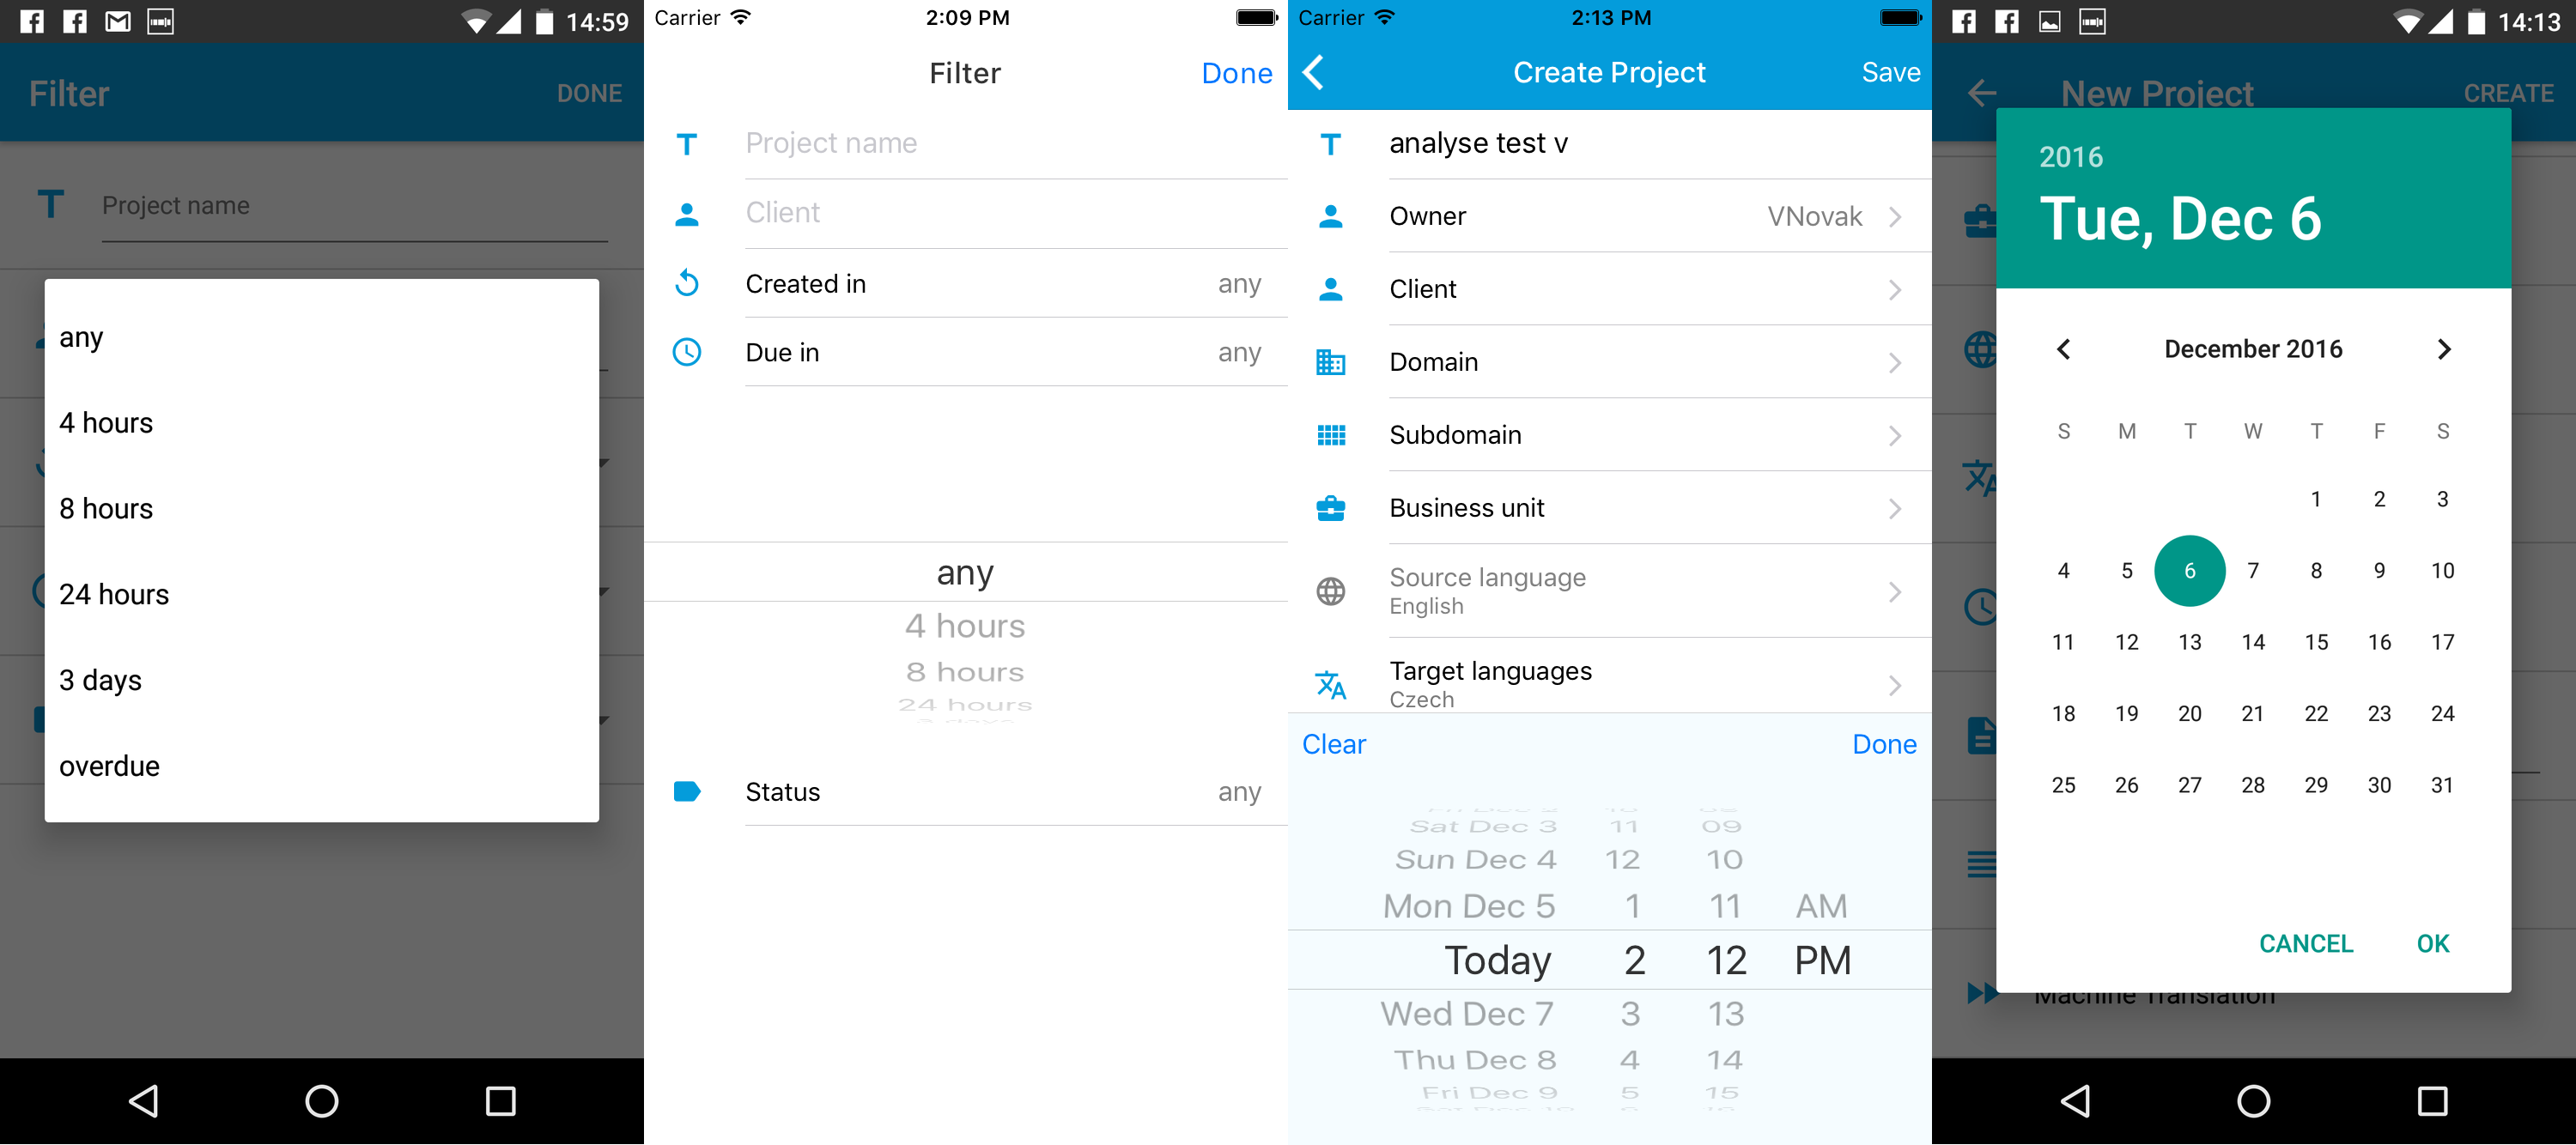
\includegraphics[width=1\textwidth]{pics/components}
	\caption{Platform-customized behavior of list and date picker components}
	\label{components}
\end{figure}


When using such components in code, one only has to provide them with the information about the icon, the values they need to show, the mode and how they should respond to user action. The logic of how the component should be displayed and styled is hidden inside of it, with the styling being overridable. This way we can construct reusable components with platform-specific behavior.


%As described in the todo section, React native offers several ways of how to handle per-platform customizations. We will use these to provide user with the app handling they are accustomed to. Examples of places that need custom handling are actions that are included in the navbar on Android while they're shown in the bottom toolbar on iOS. Also the navigation has to look differently. 

\section{Stores}

As explained in section \ref{sec:stores}, the information about projects, jobs, and other entities in stored in domain objects, which in turn are kept in stores. It is important that there is always one instance of a particular domain object in memory, and only one instance of a store.

As an example of how a store is implemented, let's consider the project store. In its constructor it accepts (among other) the user store - that way we can clean and refresh the project list in case the active user changes. It also receives apiCaller instance which is used for communication with Memsource API. Projects are stored in a Map, which is typically backed by a hash table that offers constant access time, or by other mechanism that provides sublinear access time. The keys of the Map are projects ids and the values are instances of Project class. That way we can access the stored project instances quickly. This is especially convenient because the projects are displayed in multiple tabs that correspond to filters in Memsource Cloud (all, in progress, overdue, my). One project may be displayed in any number of tabs and even when a project is displayed in all four of them, internally this refers to the same project instance. The advantage of using Map is if we receive a project, we can quickly see whether or not we already have it stored.


\subsection{Connecting Stores with Views}

Clearly, stores need to be made available to React, so that components can visualize the content of the domain objects. For this purpose, the \texttt{mobx-react} package offers the \texttt{Provider} component and inject decorator, thanks to which arbitrary objects can be passed to React components as props. 

As I explained earlier, React app is composed of a tree of components where props are passed from top to bottom. You can either pass the stores as props explicitly through the entire tree which can get tedious, or use Provider, and grant store access for them by using inject. This makes it simple and transparent to "connect" components with relevant parts of the state. Listing \ref{code:provider} shows a simple example of how color prop can be injected. We can still pass the prop explicitly from the parent component, in which case the explicit prop takes precedence. This can be taken advantage of in testing.

\lstinputlisting[label=code:provider,caption=Using MobX Provider and inject]{./code/provider.js}


\section{Upload Module}
Upload module is a native module made to allow users to upload files to Memsource Cloud and create jobs from them. It offers different ways to select the files and allows to set up various import options. After the upload is triggered, a new item representing the ongoing upload is added to the job list. A notification and a network activity indicator on Android and on iOS, respectively, inform the user of the upload status. 

There are important differences in the iOS and Android implementations, but both expose the same interfaces to the JavaScript layer. When talking about file handling in the native module, I will use the singular form for simplicity, but note the upload module has capabilities for uploading multiple files.



\subsection{Android}
To upload a file as a job, user has to either start the app and navigate to the “add job” screen and select the files for upload from a file picker, or start the app "externally" by opening a file using the Memsource app, for example from the Gmail app or a file browser. 
In both cases, the app receives a uri which points to the file. Note that the file doesn't necessarily need to be on the device, it may as well come from a cloud storage such as OneDrive or Google Drive. The user then sets up various options for the import and taps the “send” button. 
Upon pressing the button, the necessary information consisting of the selected file, upload URL and token is passed to the upload module and upload is started. At the same time, a new item is added to the job list. This item is displayed at the top of the list and, along with a notification, informs user of the running upload.


The module runs a background service whose responsibilities are issuing a notification when the upload starts, when the job is imported or if there was an error. To upload a file, we first need to check whether it is present on the device. If not, file is downloaded using the Storage Access Framework API introduced in Android 4.4. The next step is uploading the file to Memsource and creating a job from it. This is done through  the \texttt{Create New Job} API call which handles the upload and puts the file into a queue where it waits for import. A server backend service dequeues the file and creates a job from it. Because dequeuing and job creation can potentially be long-running operations, the API call returns an ID of the enqueued object immediately after the upload is finished. The Android service then repeatedly polls the \texttt{Asynchronous API} to check the status of the job that is being created. 

Once done, it issues a final notification or, if the user checked the pre-translation checkbox at job upload screen, continues with pre-translation based on project settings. This is another operation that can possibly be long-running and the native module keeps polling the \texttt{Asynchronous API} to check the pre-translation status until it is confirmed. At that point it issues the final notification.


The service repeats its download and upload requests if there was an error and is also made to run in the background so that its actions are not disrupted in case the user switches to a different app or even “kills” the app by swiping it away from the screen. The upload service also stores the results of uploads in SharedPreferences so that the application can be updated when it is killed and the job creation finishes in background.
If the app is still running at the time when the job creation is confirmed, an event is sent to JavaScript and the views are updated. If that is not the case, the response of job creation is processed the next time the app is started. If creation was successful the item which was previously added to the top of the job list is removed and the job data is re-fetched. In case of an error, the item is not removed but instead gives user an option to repeat the upload. The native module is written in Java. 
 

\subsection{iOS}
On iOS, the module provides the same functionality but behaves very differently internally. iOS is much stricter about how background tasks are handled. There are fewer things that needs to be taken care of by the developer and more that are taken care of by iOS. This gives the developer a lot less flexibility (this also resulted in a problem with the API) but also results in less coding. The job creation on iOS works in the following way: similarly to Android, files can be selected within the app or sent to the app from an outside application such as iCloud. If a file is selected using the Document Picker, iOS automatically downloads (if needed) and saves it to the app’s sandbox from where it is removed when the application exits. In case of importing the file from other application such as Mail, the file is copied to app's sandbox and the application receives the url of the file. In the latter case, removing the file is the developer's responsibility.

Originally, I wanted to use the same approach for creating job as on Android, but it turned out not to be suitable because it is not possible to upload a file using the \texttt{multipart/form-data} request; a file uploaded by iOS's background upload task is sent directly in the body of the request and having a custom request body is impossible unless we write it directly into the file (which cannot be considered a good practice). Possible workaround here is to use another Memsource API, the File API which allows to upload a file in the request body and returns a file ID which can be used in other API calls. The problem with this approach is that we would need to make two api calls to make the job import happen: first to upload the file and second to call the Create Job api. This poses a possible issue since iOS may decide to not perform our background request. 

iOS uses several pieces of information to decide whether or not a request will be carried out. The decision involves eg. how of often the app is used by the phone's owner or what the battery level is. The exact algorithm is not publicly available. It may therefore happen that the first request for file upload will be honored but the second request for actually creating the job may be ignored. The best possible solution to this is implementing another API which would accept the file in the request body and the numerous parameters sent to the the create job api would be sent as a json string in a special request header. For the time being, I have implemented the described workaround and a better solution on the server side may be implemented later. 


Similarly to Android, as the upload starts, all of its information including the user who started the upload and the project ID is serialized and stored to UserPreferences entry and is updated whenever the status of the upload or import changes. This way the information is not lost when the app is killed during or after the import and the information about whether an upload was successful can be processed the next time the app starts: if the import was requested on the server, the job entry is removed from the job list. If the upload did not finish or if the import wasn't requested, the item is kept in the list and flagged it as a failed import. The iOS native module is written in Swift 3.


\section{State Persistence}

One of the implemented features is having parts of the app's data stored on the device so that it is available right after the app’s startup. This includes information related to projects, so that when the app starts, the user sees their projects immediately, along with a loading indicator which denotes that the projects are being refreshed. MobX itself doesn't come with a mechanism for state persistence, and therefore another library, Serializr was used. Serializr provides a variety of functions for serializing data stored in different data structures and also custom objects. The data that needs to be serialized and the data structure used are described using decorators placed on the member variables of selected classes. The application also stores search history for all of its users. 

While the implemented serialization works well, it poses extra level of complexity; implementing it was a lengthy task partly due to some hard-to-find unexpected behaviors and unhelpful error messages. The (de)serialization, however, is implemented in such way that when an error happens (which is more likely to happen during deserialization), the app falls back to to not deserializing any data and instead loads the data only from the api.


State is serialized upon switching the app into the background. Serializr outputs a json object which is persisted using React Native’s AsyncStorage as a string. Note that storage of user credentials is handled differently and is described in the next section. Upon app start, the objects that hold state are created empty, the json string is deserialized and and all of the information is inserted back into the state objects through setters. 


\subsection{Storing User Credentials}

Communication with the Memsource API requires the user to enter their username and password. The app then asks for a token which is used for the requests to follow. The token validity is limited to 24 hours and the app therefore needs to request a new one once the current token's validity is approaching its expiration date. To be able to ask for a new token, the app needs to have the user credentials at its disposal, and persist them so that it doesn't need to repeatedly ask the user to enter them. Such storage, obviously, needs to be safe and the AsyncStorage used for state persistence does not meet the safety criteria. To store the user credentials, I used a package which internally uses Keychain on iOS and an encrypted SharedPreferences entry on Android. I authored the Android part of the package which is now available as react-native-keychain on npm. 

\section{Data Fetching}

Application fetches all data through the publicly available Memsource REST API, whose relevant parts used in the application are attached in appendix. The data is provided in JSON (JavaScript Object Notation) which makes it easy to work with, given that the app is written in JavaScript. The API uses standard HTTP response codes to denote operation result and provides error description when a request is incorrect.

There are some common patterns related to data fetching arising throughout the app. In many places we need to display some data, be able to reload it (using the well known pull down gesture), and be able to load more of the content and append it to the existing data (informally known as infinite loading).

Many of the used APIs use paging, ie. they deliver results in batches of 50 items per request (or less if more aren't available). The app uses this fact to find out if more items can be fetched since the number of the next page to be fetched can be calculated as $next = number \;of\; received \;items / 50$. If a response contains less than 50 items we know there are no more items to be fetched. However, we need to keep in mind that items can be both added and removed to the lists, for example when projects are added. That would give us a page number which is not an integer. In that case we perform a request for a page whose number is the closest lower integer. This may give us items that are already stored in the list, in which case we remove items at indices from $next \cdot 50$ to the end. That way we display the correct data and do not need to make any additional requests.

Also, in some cases we want to limit the number of pages that we fetch so that we do not allow the app to keep too many objects in memory which could cause undesired behavior. 

In some places where data is fetched we want to give the user a possibility to refresh the loaded list (such as in project or job lists) while in other we only offer listing without refreshing. This means we need to control up to two loading indicators that will denote refreshing (that would be the pull down indicator) or loading more content (loading indicator at the bottom of a list). We also need a means for blocking a request if it is already in progress or if is forbidden (because of reaching the limit of number of fetched items or because no more items are available). 

Blocking a request if it already in progress is needed for cases when we eg. scroll down a ListView which has the infinite loading implemented. Infinite loading is implemented using ListView’s onLoadMore function. This function is invoked when a user scrolls down the ListView and arrives at some pre-defined distance from the end of its content. Invocation of this function triggers fetching more items. In case of a poor network connection, fetching might take several seconds during which the user may scroll through the already rendered items and trigger another fetch. We need to prevent this second fetch from happening, otherwise when the returned promise resolves, it would append the results to the end of the list two or more times, causing duplicate entries.
 
If we want to have some universal fetching mechanism, it needs to account for all of these requirements. For this purpose I implemented the ProjectDetailsFetcher module. The most important function it exposes is the fetchProjectDetail function which accepts a project for which it fetches the detail (jobs, translation memories and term bases or other potential items). The other parameters include the field name (eg. jobs), a boolean denoting whether the request is a full reload request (one triggered by the pull down gesture), configuration object (eg. to specify a filter) and page limit that will not allow fetching more than specified number of pages.
ProjectDetailsFetcher internally handles the number of the next page that should be requested for a particular project and property as well as tracking which requests are allowed or not. The fetchProjectDetail function returns a Promise which contains the response data. This data is usually requested from stores. ProjectDetailsFetcher does not handle displaying or hiding the loading indicators, as I have found it to be better to control this from the places where fetching is being requested because it offers more flexibility.




\subsection{Handling Internet Connection Outage}

The application’s functionality is dependent on Internet connection since acquiring all of its data and possible user actions need access to the Memsource API. However, once the application fetches its data, it, of course, stays in the memory and is available for reading. Moreover, the app serializes data which is needed to display the list of projects and the project info screen, which includes projects, clients, domains, subdomains, business units and other details. That way the data is available for reading even if the user starts the app without Internet connection. Moreover, even if internet connection is available, user can see their projects right upon the app's start, along with a loading indicator that denotes refreshing.


When the app is offline, there is a bar displayed at the top of the screen, and it informs the user there is no Internet access. Also, when a user's request times out, they are informed about it via a toast. This behavior however, may change if I find it too intrusive. 


\section{Multi-stage deployment and testing}


One of the advantages of using React Native or hybrid application frameworks is the ability to use services such as Code Push that enable the developer to update the application without going through Apple AppStore or Google Play Store submission process. This is achieved through being able to switch the JavaScript bundle which contains the app’s logic for another one. When a developer wants to publish a new version of the app they create a new JavaScript bundle and upload it to a Code Push server. 
When a user starts the app, it downloads the new bundle (if available) and stores it. In a typical scenario, the bundle would be applied upon the next app start but this is configurable. This way the user receives updates without any interruption on their side. This does not only give us the ability to publish updates at an arbitrary frequency but also offers greater control over the updates, since the user does not influence them.


In the app, I have used the Code Push service which is being developed by Microsoft and currently offered free of charge. 


Other benefits this brings and that I have implemented is multi-stage deployment and testing. For the purposes of our app, three build configurations were set up: debug configuration where code-push is not being used; this configuration is used for everyday development and runs in React Native’s Dev mode.

The second configuration is Staging, which is set up to request the staging version of the JavaScript bundle from Code Push and uses Memsource’s pre-release server at \texttt{cloud 9.memsource.com} to serve its requests. This version is made for testing the application's new features and also its compatibility with the Memsource Cloud version which is the next to be deployed to production. The development mode is not enabled in this configuration and thus the development warnings are not shown. 


Finally, the third setup is for release. This configuration uses the corresponding JavaScript bundle from Code Push to get its updates and is identical with the staging version, with the exception of not having the latest updates that are being tested in staging. This is the version that runs on the phones of the Memsource’s customers. When suitable, the updates made in the staging version can be easily promoted to the release build of the application by a single cli command.

\section{Code Quality Tools}

Due to JavaScript's dynamic nature and the absence of any transformation that would take place before the code starts its execution, it is relatively easy to introduce bugs that only come to light during runtime. There are, however, tools for code quality assurance that help developers find potential bugs before the code is executed. In this project, I have used two such tools which this section shortly describes.

\subsection{Flow - Static Type Checker}

Flow is a static type checker for JavaScript developed by Facebook. It works by using type inference even on plain JavaScript code without any annotations by tracking the type of variables as they are used through the program. Flow therefore allows developer to catch bugs before they run the program, without changing the existing code. 

Flow attempts to infer the types whenever possible, but some JavaScript code can be very dynamic and hard to analyze statically. Flow therefore offers ways to specify types explicitly which also works as a documentation for the developer and for an IDE which can offer a better autocomplete.

Flow supports standard primitive types such as number or string, as well as custom types eg. for application-specific objects. It guards common bugs such as null dereferencing, silent type conversions and many more potential sources of bugs. An example of how flow-typed code can look like, see listing \ref{code:flow}. In this example, Flow would report that the annotated return type of \texttt{string} is incompatible with the return of the \texttt{length} function, which is a \texttt{number}. The listing also shows how to enable Flow checking for a JavaScript module --- simply include \texttt{@flow} in a comment at the top of the file.


\lstinputlisting[label=code:flow,caption=Flow-annotated JavaScript code]{./code/flow.js}

One of very useful features of Flow are maybe types which are denoted by a question mark (eg. \texttt{?string}). When accessing a function or property on an object which is of maybe type, Flow will issue a warning that \texttt{Property cannot be accessed on possibly null or undefined value}. This greatly helps avoiding the "Undefined is not an object" error which is one of the most common ones in JavaScript development. Other handy features include interfaces or guarding that a function doesn't receive too few or too many parameters. I have used Flow extensively throughout the project.

\subsection{ESLint}

ESLint is a linter -- a tool that flags potential problems in source code. ESLint takes the form of a set of rules that the developer specifies and ESLint warns her when the code violates a particular rule. Rules may describe a potential bug in source code (such as calling a function that is not defined) or a desired coding style (such as using semicolons at the end of a line).

ESLint itself does not force any rules onto the developer. Instead, different rule sets can be obtained online and plugged into the project. Choosing such rule set is often a matter of personal preference or the technology that the project uses. For example, there are React Native-specific rules that eg. warn about having unused style definitions in the component code.

todo posat vysledky pouziti. problem v js je toto, reseni je toho, pouzil jsem to takto

\section{Navigation}

By navigation, in the context of React Native, I mean transitioning between different screens of the app. Navigation integrates with the components and also stores very closely, because many parts of the code will want to navigate to a different component as a response to user input or network event, so the navigation solution is of great importance. 

RN started off with two solutions for navigation - the Navigator and NavigatorIOS. Navigator is implemented entirely in JavaScript, runs on both platforms and tries to mimic the appearance of native navigation, while NavigatorIOS leverages the native navigation of iOS.
They originally started as two competing implementations solving the same problem (todo ref) with the goal of assessing which of the two solutions should be supported further on. Ultimately, the Navigator solution was found to be better for reasons described later on, and Facebook used it in the F8 and Facebook ads applications. 


There is one notable drawback to Navigator - it is only trying to mimic the native navigation. This includes navigation bar with its animations, as well as transitions to and from different scenes of the app and implementation of the swipe back gesture. This, to a certain extent, can negative affect the user experience.
Having navigation controlled by JavaScript has its benefits - most importantly it allows for complete control of the navigation state, while with NavigatorIOS, some information sent from JavaScript to the native layer gets stored in the native code where it is managed by iOS internally which makes it hard to keep the information in JavaScript up to date. The difficulty of keeping JavaScript in sync with iOS and the fact it only works on one platform were the main reasons why Facebook decided to favor the Navigator.

Some would say that not using the native navigation breaks the promise of React Native - that is to be able to create apps that are indistinguishable from native ones. This is why Wix (an Israeli mobile and web development company) is working on a native navigation for react native. At the time of writing, there is not a stable release of this package available which is why I didn't use it.

Over the course of time new issues with using Navigator emerged and there was a need to come up with a better way of managing the navigation state. For example, the original Navigator becomes hard to work with in case we use several instances of it. For example, the application I have developed uses three different navigation components - one StackNavigation as a root navigator. The root navigator contains another StackNavigation where the vast majority of the app's content is pushed. In some places, however, I wanted to display modal windows. The modals are pushed onto the master navigator so that they are displayed in the foreground. The modal window contains another StackNavigation of its own, which yields a total of three navigators, but for applications that use a tab-based navigation or drawer navigation, that number is very likely higher. 


At the time when I started working on the project, the new solution to navigation was already present in the RN core and was named NavigationExperimental. However, since NavigationExperimental is only a set of low-level components, people started writing libraries around them to provide a more feature-rich experience for the developers. In the end, I have settled with a library called ex-navigation. It offers some needed functionality out of the box and allows to customize the behavior for iOS and Android such as handling the navigation bar, animations and back gesture on iOS as well as the back button handling on Android. Most importantly it works well with several navigators which can be managed independently and offers better animation performance - on Android, the animations are controlled from the native layer.

\section{Issues}

There were a number of issues encountered throughout the development, caused by different factors such as React Native's immaturity and frequent releases where new version is shipped every other week and updating is not always straightforward due to breaking changes (although this is changing to one release per month as of January 2017), lack of quality documentation, or my effort to create partially different UIs on each platform so that the user experience is on par with what the user would get in an application designed specifically for iOS or Android. This sometimes led to dead ends such as when I had to replace the entire navigation solution for a new one. Navigation as a whole is an interesting topic, which is why I devoted an entire section to it.
Another issue is minor differences in behavior on each platform -- the component appearance on iOS may not always be the same as the one on Android. This involves borders, border radius or animations. However, given React Native's complexity --- the library uses JavaScript, Java, Objective-C, C++ and also C --- it does a very good job in abstracting the platform away.
Other very painful issue, although visible only when rendering large UIs, are animations which are controlled from the JavaScript thread. This means that the JavaScript thread has to periodically send commands to the native layer for the animation to run. If the JavaScript thread has too much work on it, issuing the command is delayed and the result is a laggy animation. This issue, however, is already partially solved and offloading the animations from the JavaScript thready will probably be fully functional in the first months of 2017.

Other difficulties were met in working with files (uploading and downloading jobs), since this needed to be done once for each platform and involved coding in Java as well as Objective C and Swift. Working with files has many hidden culprits given by different behavior on older Android versions, file permission issues and problems resulting from different file sources - ie. files imported from other applications vs form UIDocumentPicker on iOS.
%Also, the fact that React Native is not a framework gives developer the freedom to do things in different ways, which also means that the first way a developer reaches for does not always turn out to be the best one. 


\section{Open Source Software Contributions}

Throughout the development of the application, I have contributed to different projects by bug fixes or code and documentation improvements. The projects include: 


\begin{itemize}
\item react-native-keychain
\item mobx-utils
\item react-native-scrollable-tab-view
\item ex-navigation
\item react-native-router-flux
\item serializr
\item mobx
\item react-native
\item react-native-android-kit
\item react-native-radio-button-android
\item react-native-android-checkbox
\end{itemize}


\chapter{Testing and Crash Reporting}

The Android and iOS versions of the application were implemented in parallel, mostly on my personal machine with Ubuntu 16.04 and my Nexus 5 phone with Android 6.0.1, following a verification and fine-tuning for iOS. The development phone for iOS was iPhone 5C running the latest version of iOS which was available at the time. 

I have also used the iPhone and Android emulators for development and to see how the application looks with different screen resolutions and OS versions (the latter is especially relevant for Android). However, having access to real devices was crucial, since only a real device can give a feeling of how well touchable elements respond to touches, how the software keyboard influences the displayed content and how the application functions in terms of performance. A real iPhone device was also needed for implementing the native module for creating jobs, since the background capabilities of NSURLSession of an iPhone emulator do not fully correspond to the behavior of a real device.

All throughout the development, the application was receiving its data from Memsource servers, ie. I have not used any server implementation specifically for the development.


\section{Unit Testing}
The lowest level upon which the application is tested is unit testing. I have chosen Jest \footnote{http://facebook.github.io/jest/} for implementing the unit tests. Jest, like several other tools I have used, is a library actively developed by Facebook and is open source. 

It offers essential functionality similar to other popular JavaScript test runners (e.g. AVA or Mocha), such as making assertions upon the results of tested code, creating mocks and also offers snapshot testing, which is functionality that can be used for testing the structure of React trees (or any serializable values) without directly rendering them. Snapshot testing is a very useful feature especially in React Native as it allows to test component appearance without the need for rendering the UI on a device or emulator. 

Jest creates a snapshot that captures the necessary information for component rendering. When the component changes, the snapshot changes as well, and we're notified of this fact during testing. If the change is intentional, we can simply overwrite the previous snapshot with a new one, or fix the problem if the change is a bug. We also see the change in version control when the it is being merged since the snapshot files live alongside the code. Snapshot testing also can be used for testing application state.

Snapshot testing currently has the drawback of not being able to trigger and capture possible changes in the inner state of the component (if there is any state), ie. snapshot testing only considers the component’s props. This, however, is a subject to change in one of the future releases of Jest.

Since a React Native app is a native application, we can use the same testing frameworks that we would use for testing any other native app on ios or Android. 

todo popsat kolik jich ej jak jsem je pouzil atd - vystupy

% TODO heuristic evaluation

\section{Testing With Users}

I performed informal testing of the Android application with three users all of whom were Android users. One was a user knowledgeable of Memsource in general but not its advanced features, second was a Memsource power user and third was a novice user. They were given a sheet with tasks (available in \autoref{chap:walkthrough}) they were asked to perform using the mobile application.

During the test I was, for the most part, just silently observing the user actions but also communicated with user when they wanted to tell me something. This section contains the outputs of the tests with my comments included. I also made a summary of the encountered problems.


\subsubsection{First Test (knowledgeable user)}

In the first test, all tasks were completed. The test revealed some inconsistencies in how project metadata is presented in the project info screen. User also reported that the control for selecting linguist (in the screen for creating new jobs) doesn’t seem to be a control that would react to touch (button), plus the heading which reads "select linguists" is not intuitive. 

Next, I observed that the user expected something (item selection) to happen when they tapped an item in the job list. The user got around it by long-pressing the item, which is the intended way of selecting it. The selection logic was implemented at a time when there was another action expected to happen upon short tap (a preview of the imported job). This functionality was decided not to be needed in the end. I have later implemented a fix for this - the short as well as long taps are now used for item selection. 


When selecting Term Bases (TBs) and Translation Memories (TMs), the user was slightly confused by the term "Selected TMs". I agree a better term would be "Attached TMs" as was suggested, but chose the term "Selected TMs" to keep consistency with Memsource Cloud. The user also found the screen for adding TMs and TBs generally confusing. This is due to too many controls being displayed on one screen (a control for filtering the results, control for selecting the target language and workflow step for the assignment, along with checkboxes and dialogs for selecting different parameters). This problem was later addressed by splitting the adding of TMs and TBs into two screens, so it now involves an extra step, but is much clearer.


\subsubsection{Second Test (power user)}

In the second test, all tasks were completed as well. The second user performed the project and job tasks successfully. They also found an unexpected text reading "owner from different organization" on some project items displayed in the project list. This is an older issue caused by the API not returning the project owner. It remained in the application since I forgot to investigate the root cause. At any rate, the message looks confusing and will be removed and I will look more into the cause and possible solutions. The user also requested one feature and noticed one bug, both relating to content displayed in the project info screen.

Similar to the first test, I observed the user was confused when adding TMs because of they expected that the TMs in the screen that lists them to react to touches, while the listing is intended as a read-only preview. I later addressed this problem by adding an "edit" button in the navigation bar but it still remains to be assessed whether this is a sufficient improvement.

The user also reported confusion over the fact that when TBs are added for language X, the "Selected TBs" section shows TBs selected also for other languages. This is something I need to think through and the solution to this perhaps lays at the server side which provides this data.

%Show date created in project info screen
%Workflow steps not always shown in proj info screen

\subsubsection{Third Test (novice)}

The third test was also completed successfully. The app already included the aforementioned fixes to how jobs are selected and how TM and TB selection is split into two steps which both made completing the tasks easier for the user. 

User had the following remarks to the application: when only one job is selected for editing, the edited fields read "leave unchanged" while they could read the actual data of the edited job, and "leave unchanged" should only be used when multiple jobs are being edited. This is certainly true and may be implemented. 

User also didn't like that the very general "no results" text is shown when an empty list of jobs, TMs or TBs is displayed. User would appreciate more specific messages. This is a simple to do improvement and will be implemented.

Another thing the user was confused about were the icons for searching (magnifying glass) and filtering (funnel). This is something not very easy to address, since searching and filtering are very similar, yet different tasks.

Same as in previous tests, user had complaints about how TM and TB selection works --- the user didn't like that some items are being selected and de-selected automatically.

My last observation from this test is that the user wasn't sure how to trigger the search after entering the search phrase in the text box. This is done through a key located in the lower right corner of the screen, which shows a magnifying glass. The icon, however, is rather small and therefore not always easy to notice. User found the button after a few seconds and managed to trigger the search but said they expected the search to happen as they type. This is something we will consider for later implementation.

\subsection{Test Conclusions}

The tests of the application for Android were completed by all users. Unfortunately I didn't manage to run a user test with the iOS version of the application. The tasks related to projects and jobs were completed by all users without problems. Issues emerged when attaching Translation Memories and Term Bases to the project. This is due to the way items are presented for selection. I have already addressed some of these issues and will continue working on them.

The way TMs and TBs are selected can be further improved. Now, while the mobile app is consistent with Memsource Cloud, I find it somewhat confusing (and the tests confirmed it): when the user selects eg. a TM in read more, write mode is automatically selected too and user is not always in complete control. Not all checkboxes that seem to be possible to select can be selected due to selection constraints.

I believe a better solution to the problem is a single button reading something like “select TM (TB) mode”, which would open a list with all possible modes for the TM (TB) and only one mode could be selected. The list would show all modes: “Read \& Write”, “Read only” in case of TMs and in case of TBs “Read \& Write”, “Read \& write \& QA”, “Read only”, “Read \& QA”. If applicable, the modes would be displayed along with an explanation of why a particular mode cannot be selected, or that selecting the mode will overwrite the mode of some other TM (TB). This would give user complete control and no unexpected automatic selecting or de-selecting happening as it is now.


\section{Crash Reporting}


One of the requirements is the ability to collect crash reports from users running the application so that we can observe how it functions on their devices and react to potential issues. 

There are several services which provide crash reporting as well as means for collecting information about how the app is used, similar to analytics as it is on the web. One of such solutions which is widely used and also has community-developed bindings for React Native is called Fabric \footnote{https://get.fabric.io/} and is provided by Twitter free of charge for both iOS and Android. Fabric's crash reporting service is called Crashlytics, and the analytics is marketed under the name Answers. I have chosen Fabric because of its popularity, the ability to use Crashlytics as well as Answers and the fact it is available for both platforms. I have incorporated Fabric into both Android and iOS versions of the app. 

While Fabric with the community-developed module for React Native does report the application crashes, I am not completely happy with how the reported issues are presented in the Crashlytics dashboard. In particular, when a crash happens in the JavaScript layer of the application, the information is merely passed to the native module which backs the JavaScript module. In the native module, an exception is thrown and its information is collected and recorded by Crashlytics. The problem with this approach is that all exceptions are thrown from exactly the same line in code and Crashlytics considers all of them to relate to a single bug. Then, in the Crashlytics dashboard (which is best accessible though web browser) all of the exceptions are grouped together which makes working with Crashlytics uncomfortable. I have investigated other possible crash reporting solutions and found Bugsnag \footnote{https://bugsnag.com/} which directly supports React Native. It, however, does not provide any analytics service and is not offered free of charge. I will evaluate the situation around bug reporting after we gain more experience with Crashlytics and might make a switch.

\chapter{Conclusions and Future Work}

Mobile devices are ubiquitous and people use them extensively in their everyday lives. As a consequence, many online services are accessible not only through the web, but also via applications made specifically for mobile devices. Indeed, the presence of mobile devices is so strong that many products are even built solely for mobile and do not exist on the desktop.

Memsource Cloud is an online service that had no mobile application and the goal of this thesis was to change it. In the its scope I have introduced Memsource to the reader and explained the motivation. Since it was clear from the beginning that the application must be multiplatform, I have performed an analysis and comparison of the tools for multiplatform development. Prior to starting the development I have collected requirements for the application and created mockups at different fidelity levels. The application was implemented mostly in JavaScript and React, with Swift, Objective C and Java being used in the functionality implemented natively. 

I have laid the foundations for an application that will allow Memsource users access the most important features of Memsource Cloud. The current functionality includes CRUD operations on projects and jobs, as well as working with term bases and translation memories and other features.

What I have not managed to implement, are features for linguists because it turned out an API was not available for what I thought was a very simple matter. The API is to be developed and adding the features for linguists should be simple, as they are already implemented for the project manager role.

React Native, despite its young age proved to be a valuable and functional library for multiplatform mobile app development, albeit sometimes it required a little more work than I'd like to make things work exactly the way I wanted. Its easy integration with the underlying platform was important for working with files in the native modules. Also MobX is a library that works very well with React and I have enjoyed working with.


The future work will involve further development of the application within Memsource. I will continue adding more features to the application, and improve the styling of some components. Another important future step is to introduce a continuous integration tool.



\appendix

\chapter{Tasks for Testing with Users}
\label{chap:walkthrough}

Log in with the following credentials: username “VNovak” and password (removed). You will be presented with the list of all your projects which are shown in different tabs.

\subsubsection{Projects}

Take a look around and familiarize yourself with the screen. When you’re ready, create a new translation project with the following parameters: 

\begin{itemize}
\item project name: “yet another project”
\item Client: Slavia
\item Domain: Machinery
\item Source language: English 
\item Target languages: Czech, German
\item Due date: 19th of January at 7 pm
\item Workflow steps: select translation and revision
\end{itemize}


Verify the created project and try to list jobs of the project. The list should be empty at this time. 


\subsubsection{Jobs}

Now let’s create a new job in the project. The job should be created from a file named “important document.doc” which is present in the device's Google Drive found under “mobile app/testfiles”. 
Keep the job’s target languages se to “cs” and “de”.
Set the job’s due date to 11th of January, 10 am and select the “VNovak23“ user as the linguist for both languages. 
Make sure that comments and hidden text from the word document are imported and then create the job. 

Wait for the job to be imported and then list the jobs and switch to the “Revision” workflow step. Select the job part whose target language is German and change its due date to 17.1.2017 11 am and save. Verify the due date is updated.

\subsubsection{Translation Memories}

The next task is to add existing translation memories to the project. If you list the translation memories, you will see that none are assigned yet. Attach the “Software TM“ translation memory to the German target language and all workflow steps. Attach it with read and write modes enabled, a penalty of 10\%. You may use the filter if you’re having trouble finding it. For Czech, attach “HackerX TM” in both read and write mode and “interview” TM only in read mode, also for all workflow steps. Verify the translation memories are attached after saving.

\subsubsection{Term Bases}

The next step is to add term bases to all languages.
Attach the “Clock Industry” term base with read, write and QA enabled. Also add the “jim” term base in read mode. 

After the term bases are attached, go back to the project list screen and try to use the search feature to find the project you just created. Verify it shows up in the search results and that you can open it. 

That's it for today, thank you for your participation!
\chapter{Used API Calls}
The entire API documentation can be found at \href{http://wiki.memsource.com/wiki/Memsource_API#API_Reference}{''Memsource wiki''}. This appendix lists only the APIs used by the mobile application. The documentation is shown in a slightly simplified manner (without comments).

\section{Project API}

\subsection{Create Project API}

\begin{alltt}
\textbf{action: api/v3/project/create}
token                       string
name                        string                             
sourceLang                  locale
targetLang                  list(locale)
client                      domain(Client)                     O
businessUnit                domain(BusinessUnit)               O
domain                      domain(Domain)                     O
subDomain                   domain(SubDomain)                  O
dateDue                     datetime                           O
note                        string                             O
machineTranslateSettings    domain(MachineTranslateSettings)   O
workflowStep                list(domain(WorkflowStep))         O
useDefaultProjectSettings   boolean                            O

\textbf{response: JSON}
\{
	"id": 238                
\}
\end{alltt}


\subsection{Create New Project From Template}
\begin{alltt}
\textbf{action: api/v3/project/createFromTemplate}
token                       string
template                    domain(ProjectTemplate)
name                        string                             
dateDue                     datetime                           O
note                        string                             O
sourceLang                  string                             O
targetLang                  list(string)                       O
workflowStep                list(domain(WorkflowStep))         O

\textbf{response: JSON}
\{
	"id": 238                 
\}
\end{alltt}

\subsection{Edit Project}
\begin{alltt}
\textbf{action: api/v3/project/edit}
token                       string
project                     domain(Project)
name                        string                             O
status                      enum(ProjectStatus)                O
targetLang                  list(locale)                       O
client                      domain(Client)                     O N
businessUnit                domain(BusinessUnit)               O N
domain                      domain(Domain)                     O N
subDomain                   domain(SubDomain)                  O N
dateDue                     datetime                           O N
note                        string                             O N
machineTranslateSettings    domain(MachineTranslateSettings)   O N
workflowStep                list(domain(WorkflowStep))         O
owner                       domain(User)                       O

\textbf{response: empty}
\end{alltt}

\subsection{Delete Project}
\begin{alltt}
\textbf{action: api/v3/project/delete}
token                       string
project                     domain(Project)
purge                       boolean             O(false)

\textbf{response: empty}
\end{alltt}

\subsection{Get Translation Memories}
\begin{alltt}
\textbf{action: api/v3/project/getTransMemories}
token                       string
project                     domain(Project)

\textbf{response: JSON}
[
\{
	"writeMode":true,
	"transMemory":{
		"id":1,
		"targetLangs":[
		"de"
		],
		"sourceLang":"en",
		"name":"transMem"
	},
	"targetLang":"de",
	"penalty":0,
	"readMode":true,
	"workflowStep":null
\}
]
\end{alltt}

\subsection{Set Translation Memories}
\begin{alltt}
\textbf{action: api/v3/project/setTransMemories}
token                       string
project                     domain(Project)
readTransMemory             list(domain(TransMemory))  O
writeTransMemory            list(domain(TransMemory))  O
penalty                     list(double)               O
targetLang                  locale                     O
workflowStep                domain(WorkflowStep)       O

\textbf{response: empty}
\end{alltt}


\subsection{Get Term Bases}
\begin{alltt}
\textbf{action: api/v3/project/getTermBases}
token                       string
project                     domain(Project)

\textbf{response: JSON}
[
\{
	"writeMode":true,
	"termBase":{
		"id":1,
		"langs":[
		"de", "en"
		],
		"name":"termBase"
	},
	"targetLang":"de",
	"readMode":true,
	"workflowStep":null
\}
]
\end{alltt}


\subsection{Set Term Bases}
\begin{alltt}
\textbf{action: api/v3/project/setTermBases}
token                       string
project                     domain(Project)
readTermBase                list(domain(TermBase))     O
writeTermBase               domain(TermBase)           O
qualityAssuranceTermBase    list(domain(TermBase))     O
targetLang                  locale                     O

\textbf{response: empty}
\end{alltt}


\subsection{List Projects}
\begin{alltt}
\textbf{action: api/v3/project/list}
token                       string
page                        integer                    O(0)
name                        string                     O
client                      string                     O
businessUnit                string                     O
status                      list(enum(ProjectStatus))  O
targetLang                  list(locale)               O
domain                      string                     O
subDomain                   string                     O
costCenter                  string                     O
dueInHours                  integer                    O
createdInLastHours          integer                    O
sourceLang                  list(locale)               O
owner                       domain(User)               O

\textbf{response: JSON}
[
{
	"id":1,
	"uid":"cU19tI7NPTOI8y3Ot4VbE7",
	"internalId":1,
	"name":"project",
	"status":"NEW",
	"sourceLang":"en",
	"targetLangs":[
	"cs",
	"de"
	],
	"dateDue":null,
	"dateCreated":"2016-09-02T08:40:00+0000",
	"note":null,
	"machineTranslateSettings":null,
	"workflowSteps":[
	
	],
	"client":null,
	"businessUnit":{
		"id":1,
		"name":"businessUnit"
	},
	"domain":null,
	"subDomain":null,
	"langSettings":[
	
	],
	"createdBy":{
		"deleted":false,
		"active":true,
		"userName":"admin",
		"firstName":"admin",
		"id":1,
		"lastName":"test",
		"role":"ADMIN",
		"email":"test@test.com"
	},
	...(redacted)
}
]
\end{alltt}
\input{appendices/jobApi}

\printindex

\appendix



\bibliographystyle{amsalpha}
\bibliography{ctutest}

\ctutemplate{specification.as.chapter}

\end{document}